\documentclass[12pt,a4paper]{article}
\usepackage{ucebnice}

\usetikzlibrary{arrows.meta}

\title{Planimetrie}
\author{Ondřej Škubala}
\date{\today}

\begin{document}

\maketitle
\newpage

\section{Planimetrie}

\begin{historicalbox}

\textbf{Počátky geometrie}

\smallskip
Planimetrie, tedy geometrie rovinných útvarů, patří k nejstarším oblastem matematiky,
neboť její využití je úzce spojeno s praktickými potřebami člověka, jako je měření pozemků,
stavba budov a další činnosti vyžadující přesné určení tvaru a velikosti ploch.

Ještě dříve než vznikla formální geometrie, lidé používali základní geometrické principy
v praxi. Například starověcí Egypťané a Babyloňané již před tisíci lety znali
základní geometrické tvary a uměli je využívat při stavbě pyramid a měření polí.

Nejstarší doložené geometrické poznatky nacházíme ve starověkém Egyptě,
kde se geometrie rozvíjela především díky potřebě měřit a rozdělovat pozemky podél Nilu.
Které souvisely s každoročními záplavami řeky, které měnily hranice polí.
Nutnost každoročně vyznačovat hranice pozemků vedla k rozvoji základních geometrických principů.
Již toto vedlo Egypťany k rozvoji praktických metod měření délek, úhlů a obsahů.
Egypťané dokázali pracovat s jednoduchými geometrickými tvary, jako jsou čtverce,
obdélníky a trojúhelníky, a uměli vypočítat jejich obsahy. Dokonce již dokázali určitým způsobem
pracovat i s pravouhlými trojúhelníky, což je základní princip pozdějšího \textbf{Pythagorova věta}, neboli Pythagorovi věty.
Nicméně jejich poznatky nebyly systematicky uspořádány a chyběla jim teoretická podpora,
která by umožnila hlubší pochopení geometrických vztahů. Chyběla u nich empirická metoda a deduktivní logika,
které by umožnily vytvoření uceleného systému geometrických poznatků.

\bigskip
\textbf{Antické Řecko - zrod deduktivní geometrie}

\smallskip
Zásadní zlom v pojetí co to je geometrie přinesli starověcí \textbf{Řekové}.
Ti jako první začali geometrii chápat jako vědu založenou na logických důkazech a systematickém uspořádání poznatků.
A zároveň i jako určitou formu filozofie, která zkoumá povahu prostoru a vztahy mezi geometrickými objekty.

Prvním z těchto \emph{myslitelů} byl \textbf{Thales z Milétu} (asi 624–546 př. n. l.),
který je považován za zakladatele řecké geometrie. Jsou mu připisovány první geometrické věty a jejich důkazy,
například \emph{věta o úhlu v polokruhu}. Tímto položil základ myšlence,
že geometrické poznatky musí být logicky odvoditelné z obecných principů \emph{přijaté předpoklady – axiom}.

Nejvýznamnějším řeckým matematikem byl však \textbf{Eukleidés} (asi 300 př. n. l.),
který je často označován jako \emph{otec geometrie}. Vrcholem celé antické geometrie
je právě jeho dílo \textbf{Základy - Elementa}, které systematicky shrnuje veškeré tehdejší geometrické poznatky.
Eukleidés zavedl pojem \emph{axiomů} a \emph{definic}, ze kterých odvozoval další geometrické věty pomocí logických důkazů.
V jeho díle najdeme jak axiomy, postuláty, tak i nedefinovatelné pojmy.
Pomocí logické dedukce odvozoval vlastnosti \textbf{bodů}, \textbf{přímek} a \textbf{úhlů}, tak i vztahy mezi nimi.
Tyto jeho definice a věty tvořili a stále tvoří základní stavební kameny planimetrie, po více jak 2000 letech (see how bad ass he was?).
% pět postulátů - neukleidovská geometrie
V jeho díle taktéž můžeme najít i pět postulátů (axiomů):
\begin{itemize}
    \item Dvěma body lze vést přímku
    \item Přímku lze neomezeně prodlužovat
    \item Ze zadaného bodu lze opsat kružnici se zadaným poloměrem
    \item Všechny pravé úhly jsou stejné
    \item Pokud dvě přímky protínají třetí tak, že součet vnitřních úhlů na jedné straně je menší než dvě pravé úhly, pak se tyto přímky na této straně protínají
\end{itemize}

Všechny postuláty až na ten pátý se zdáli již současníkům Euklida složitý. Tento postulát byl dokázán
až v 19. století, kdy matematici, jako \textbf{Carl Friedrich Gauss}, \textbf{Nikolaj Ivanovič Lobačevskij} a
\textbf{János Bolyai} uvědomili, že problém nespočívá v nedostatečné důmyslnosti důkazu, 
ale v samotném předpokladu, že pátý postulát musí platit. Nakonec se ukázalo, že lze vybudovat
zcela novou konzistentní geometrii, založenou na tomto postulátu, která se dnes nazývá \textbf{neukleidovská geometrie}.

Zároveň závádí i pojem \textbf{Eukleidovská konstrukce}, což jsou konstrukce prováděné pouze pomocí kružítka a pravítka.
Ale bez velikostí, které jsou základem planimetrie dodnes. V podstatě si to můžeme představit jako tyč a provázek,
které nám pomáhají s konstrukcí geometrických útvarů.

\bigskip
\textbf{Středověk – uchování a rozvoj geometrického poznání}

\smallskip
Po pádu Západořímské říše došlo v Evropě k úpadku vědeckého poznání, včetně geometrie.
Nicméně se alespoň v Evropě dál uchovávala a dále rozvíjela díky činnosti \textbf{klášterních škol}
a \textbf{arabských učenců}. Arabští matematici, jako \textbf{Al-Chvárizmí} a \textbf{Omar Chajjám},
přeložili a rozšířili Eukleidovo dílo a přidali k němu vlastní poznatky.
Arabové také přispěli k rozvoji geometrie zavedením nových metod a technik,
jako je například využití algebraických metod k řešení geometrických problémů.
Tyto geometrické poznatky využili v praxi a to ať už při stavbě měst, vodovodů nebo při navigaci, anebo
také pro optiku a astronomii. Díky Arabům se geometrie dostala zpět do Evropy
v době \textbf{renesance}, kdy došlo k obnovení zájmu o klasické vědy a umění.

\bigskip
\textbf{Novověk – rozvoj geometrie a její aplikace}

\smallskip
V novověku došlo k dalšímu rozvoji geometrie, a to jak v teoretické, tak i v praktické rovině.
A to především prací \textbf{René Descartes}, který propojil geometrii a algebru
a vytvořil tak \textbf{analytickou geometrii}. Tím umožnil řešení geometrických problémů pomocí algebraických rovnic
a naopak geometrické interpretace algebraických rovnic. Tento přístup otevřel nové možnosti pro studium geometrických objektů
a jejich vlastností. Právě díky Descartovi se geometrie stala nedílnou součástí moderní matematiky a
matematici jako \textbf{Isaac Newton} a \textbf{Gottfried Wilhelm Leibniz} využili geometrické principy
při vývoji \textbf{infinitesimálního počtu} (Integrální a diferenciální počet).

\bigskip
\textbf{Současnost}

\smallskip
V 19. století došlo k dalšímu významnému rozvoji geometrie, a to zejména díky objevům v oblasti neukleidovské geometrie.
Matematici jako \textbf{Bernhard Riemann} a \textbf{Felix Klein} rozšířili pojetí geometrie
a zavedli nové geometrické struktury, jako je \textbf{Riemannova geometrie} a \textbf{projektivní geometrie}.
Tyto nové přístupy umožnily studium geometrických objektů v širším kontextu a měly významný dopad na další oblasti matematiky
a fyziky, včetně \textbf{teorie relativity}.
\end{historicalbox}


\section{Úvod do planimetrie}

Geometrie patří mezi nejstarší části matematiky, která se zabývá studiem tvarů,
velikostí a vzájemných vztahů mezi geometrickými objekty. 
Jednou z nejstarších částí geometrie je \important{planimetrie}, která se konkrétně zaměřuje na rovinné útvary, 
jako jsou \textbf{body, přímky, úhly, trojúhelníky, čtverce, obdélníky} a další mnohoúhelníky.
Planimetrie se nezabývá pouze teoretickými aspekty geometrie,
ale také praktickými aplikacemi, jako je měření a konstrukce geometrických útvarů.
Planimetrie je základem pro mnoho dalších oblastí matematiky, jako je \textbf{stereometrie} (geometrie prostorových útvarů),
\textbf{trigonometrie} (studium vztahů mezi úhly a stranami v trojúhelnících) a \textbf{analytická geometrie} (geometrie založená na souřadnicích a algebraických metodách).

Planimetrie tak tvoří důležitý základ nejen pro další studium geometrie, ale i pro mnoho praktických aplikací v různých oborech, 
jako je architektura, inženýrství, fyzika a další.
Geometrické poznatky získané v planimetrii nám umožňují lépe porozumět světu kolem nás a řešit různé problémy spojené s tvary a velikostmi.
Schopnost pracovat s geometrickými objekty a chápat jejich vlastnosti je klíčová pro mnoho oblastí vědy a techniky, 
a proto je studium planimetrie nezbytnou součástí matematického vzdělávání.

V následujících kapitolách se seznámíme se základními pojmy geometrie, jako jsou jako bod, přímka, úhly a další geometrické objekty, 
a naučíme se základní vlastnosti a vztahy mezi nimi.



\section{Základní pojmy}

Každá matematická teorie začíná zavedením základních pojmů, které dále nedefinujeme,
ale přijímáme je intuitivně. V geometrii mezi tyto základní pojmy patří
\textbf{bod}, \textbf{přímka} a \textbf{rovina}.
Tyto pojmy příjmáme často dost intuitivně a jejich význam si představujeme právě pomocí geometrických obrazů.
Z těchto základních pojmů pak odvozujeme další geometrické objekty pomocí definic, 
axiomů a logických důkazů odvozujeme další, jako jsou \textbf{trojúhelníky}, \textbf{čtverce}, \textbf{obdélníky} a další mnohoúhelníky.

\subsection{Bod}
Bod je nejjednodušší geometrický objekt. Často si jej představujeme jako malou tečku, jako přesně určené místo v rovině.
Eukleidés ve svém díle \textit{Základy} definoval bod jako \emph{„to, co nemá žádnou část“}, což znamená, že bod nemá žádnou velikost, délku ani šířku.

\begin{definitionbox}
    \textbf{Bod} je to, co nemá žádnou část.
\end{definitionbox}

Bod se tak stává základním stavebním kamenem geometrie, protože všechny ostatní geometrické objekty jsou tvořeny body.
Bod obvykle označujeme velkým písmenem, například \(A\), \(B\) nebo \(C\).

%znázornění bodu jako tečky je pouze konvencí, která nám pomáhá lépe si představit tento abstraktní pojem.
\begin{center}
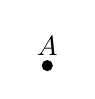
\begin{tikzpicture}[scale=1]
\fill (0,0) circle (2pt);
\node[above] at (0,0) {$A$};
\end{tikzpicture}
\end{center}


\subsection{Přímka}
Přímka je základním geometrickým objektem, který se skládá z nekonečného množství bodů, které jsou uspořádány v jedné řadě. 
Eukleidés definoval přímku jako \emph{„to, co má délku, ale nemá šířku“}, což znamená, že přímka je nekonečně dlouhá, ale nemá žádnou tloušťku.

\begin{definitionbox}
    \textbf{Přímka} je délka bez šířky.
\end{definitionbox}

Přímku obvykle označujeme malým písmenem, například \(p\), \(q\), nebo \(m\), nebo dvěma body, které leží na přímce, například \(AB\) nebo \(CD\).

\begin{center}
    \begin{tikzpicture}[scale=1]
    \draw (-3,0) -- (3,0);
    \fill (-1,0) circle (2pt);
    \fill (2,0) circle (2pt);
    \node[above] at (-1,0) {$A$};
    \node[above] at (2,0) {$B$};
    \node[below] at (0,0) {$p$};
    \end{tikzpicture}
\end{center}

V moment kdy máme dva body, lze nimi vést právě jednu přímku, což je základní axiom geometrie.
Pokud máme tři body, které všechny leží na jedné přímce, říkáme, že jsou \textbf{kolineární}. Pokud tři body neleží na jedné přímce, říkáme, že jsou \textbf{nekolineární}.

\begin{center}
    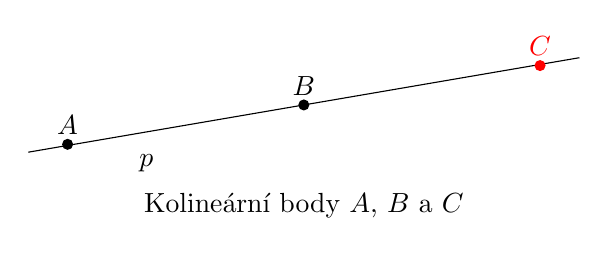
\begin{tikzpicture}
        \draw (-1.5,-0.1) -- (5.5,1.1);
        \fill (-1,0) circle (2pt);
        \fill (2,0.5) circle (2pt);
        % red dot
        \fill[red] (5,1) circle (2pt);
        \node[above] at (-1,0) {$A$};
        \node[above] at (2,0.5) {$B$};
        \node[above, red] at (5,1) {$C$};
        \node[below] at (0,0) {$p$};
        \node[below] at (2,-0.5) {Kolineární body $A$, $B$ a $C$};
    \end{tikzpicture}
    \vspace{0cm}
    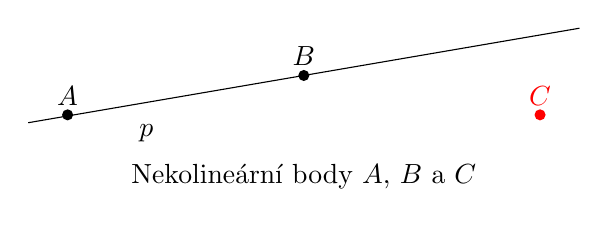
\begin{tikzpicture}
        \draw (-1.5,-0.1) -- (5.5,1.1);
        \fill (-1,0) circle (2pt);
        \fill (2,0.5) circle (2pt);
        \fill[red] (5,0) circle (2pt);
        \node[above] at (-1,0) {$A$};
        \node[above] at (2,0.5) {$B$};
        \node[above, red] at (5,0) {$C$};
        \node[below] at (0,0) {$p$};
        \node[below] at (2,-0.5) {Nekolineární body $A$, $B$ a $C$};
    \end{tikzpicture}
\end{center}

\subsection{Úsečka}
Úsečka je část přímky, která je ohraničena dvěma body, které se nazývají \textbf{koncové body} úsečky.
Úsečka se obvykle označuje dvěma velkými písmeny, které představují její koncové body, například \(AB\) nebo \(CD\).
Úsečka má délku, která je určena vzdáleností mezi jejími koncovými body. Délka úsečky se obvykle označuje malým písmenem, například \(a\) nebo \(b\).

\begin{definitionbox}
    \textbf{Úsečka} je část přímky ohraničená dvěma body, které se nazývají \textbf{koncové body} úsečky.
\end{definitionbox}

\begin{center}
    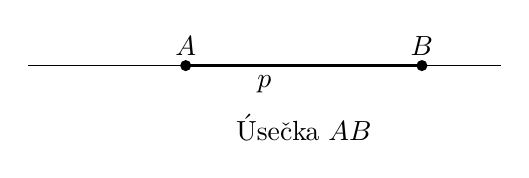
\begin{tikzpicture}[scale=1]
    \draw (-3,0) -- (3,0);
    \fill (-1,0) circle (2pt);
    \fill (2,0) circle (2pt);
    \node[above] at (-1,0) {$A$};
    \node[above] at (2,0) {$B$};
    \node[below] at (0,0) {$p$};
    \draw[thick] (-1,0) -- (2,0);
    \node[below] at (0.5,-0.5) {Úsečka $AB$};
    \end{tikzpicture}
\end{center}


\subsection{Polopřímka}
Polopřímka je část přímky, která začíná v určitém bodě, který se nazývá \textbf{počáteční bod} polopřímky, a pokračuje nekonečně daleko v jednom směru.
Polopřímka se obvykle označuje dvěma velkými písmeny, přičemž první písmeno představuje počáteční bod a druhé písmeno představuje směr, 
kterým polopřímka pokračuje, například $\overrightarrow{AB}$.

\begin{definitionbox}
    \textbf{Polopřímka} je část přímky, která začíná v určitém bodě, který se nazývá \textbf{počáteční bod} polopřímky, a pokračuje nekonečně daleko v jednom směru.
\end{definitionbox}

\begin{center}
    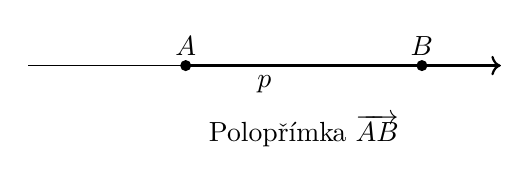
\begin{tikzpicture}[scale=1]
    \draw (-3,0) -- (3,0);
    \fill (-1,0) circle (2pt);
    \node[above] at (-1,0) {$A$};
    \fill (2,0) circle (2pt);
    \node[above] at (2,0) {$B$};
    \node[below] at (0,0) {$p$};
    \draw[thick,->] (-1,0) -- (3,0);
    \node[below] at (0.5,-0.5) {Polopřímka $\overrightarrow{AB}$};
    \end{tikzpicture}
\end{center}

\subsection{Rovina}
Rovina je základní geometrický útvar, který si představujeme jako nekonečně rozlehlou plochu bez tloušťky. 
Eukleidés definoval rovinu jako \emph{„to, jen délku a šírku má“}, což znamená, že rovina je nekonečně rozlehlá, ale nemá žádnou tloušťku.
Eukleidés tím chtěl vyjádřit, že rovina je plochý geometrický útvar, v němž všechny přímky leží \emph{rovně}.

\begin{definitionbox}
    \textbf{Rovina} má pouze délku a šířku.
\end{definitionbox}

Rovina se obvykle označuje řeckými písmeny, například \(\pi\), \(\rho\) nebo \(\alpha\).

\begin{center}
    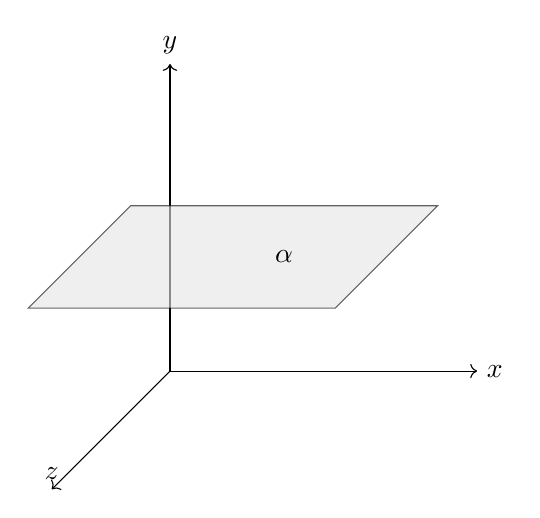
\begin{tikzpicture}[scale=1.3]
        % osy
        \draw[->] (0,0,0) -- (3,0,0) node[right] {$x$};
        \draw[->] (0,0,0) -- (0,3,0) node[above] {$y$};
        \draw[->] (0,0,0) -- (0,0,3) node[above] {$z$};

        % rovina
        \filldraw[fill=gray!20, opacity=0.6]
        (-1,1,1) -- (2,1,1) -- (3,2,1) -- (0,2,1) -- cycle;

        \node at (1.5,1.5,1) {$\alpha$};

    \end{tikzpicture}
\end{center}

\subsection{Polorovina}
Analogicky jako bod dokáže rozdělit přímku na dvě opačné polopřímky, tak přímka
rozděluje rovinu na dvě opačné \important{poloroviny}. 
Polorovina je část roviny, která je ohraničena přímkou, která se nazývá \textbf{hraniční přímka} poloroviny.
Polopřímku zapisujeme jako $\mapsto pA$, pokud přímku $p$ definujeme třeba body $X,Y$, pak se značí polorovina jako $\mapsto XYA$.

\begin{definitionbox}
    \textbf{Polorovina} je část roviny,
    která je ohraničena přímkou.
    Tuto přímku nazýváme \textbf{hraniční přímka} poloroviny.
\end{definitionbox}


\begin{center}
    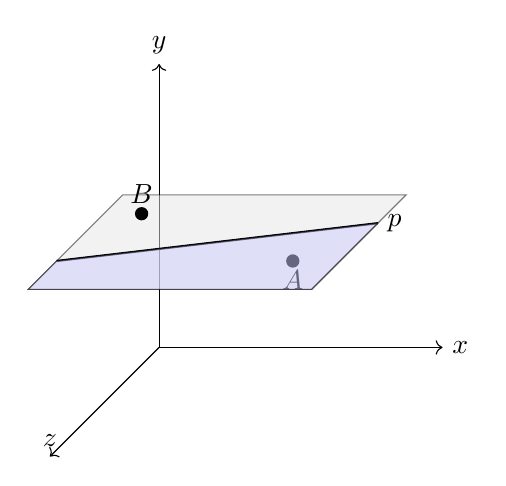
\begin{tikzpicture}[scale=1.2]
        % osy
        \draw[->] (0,0,0) -- (3,0,0) node[right] {$x$};
        \draw[->] (0,0,0) -- (0,3,0) node[above] {$y$};
        \draw[->] (0,0,0) -- (0,0,3) node[above] {$z$};
        
        % rovina alpha
        \filldraw[fill=gray!20,opacity=0.5]
        (-1,1,1) -- (2,1,1) -- (3,2,1) -- (0,2,1) -- cycle;
        
        % hraniční přímka p v rovině
        \draw[thick] (-0.7,1.3,1) -- (2.7,1.7,1);
        \node[right] at (2.7,1.7,1) {$p$};
        
        % bod A v jedné polorovině
        \fill (1.8,1.3,1) circle (2pt);
        \node[below] at (1.8,1.3,1) {$A$};
        
        % bod B v druhé polorovině
        \fill (0.2,1.8,1) circle (2pt);
        \node[above] at (0.2,1.8,1) {$B$};

        % polorovina
        \filldraw[fill=blue!20,opacity=0.5]
        (-1,1,1) -- (-0.7,1.3,1) -- (2.7,1.7,1) -- (2,1,1) -- cycle;
    \end{tikzpicture}
\end{center}
Na obrázku můžeme vidět dvě poloroviny, které jsou ohraničeny přímkou $p$.
Bod $A$ leží v jedné polorovině (modré), zatímco bod $B$ leží v druhé polorovině (šedá).


\section{Vlastnosti geometrických útvarů}
Nyní když jsme si definovali základní geometrické objekty, můžeme se zaměřit na jejich vlastnosti a vztahy mezi nimi.

\subsection{Incidence}
Pokud máme body $A$, $B$ a $C$ a přímku $p$ jako na obrázku:

\begin{center}
    \begin{tikzpicture}
        \draw (-1.5,-0.1) -- (5.5,1.1);
        \fill (-1,0) circle (2pt);
        \fill (2,0.5) circle (2pt);
        \fill (5,0) circle (2pt);
        \node[above] at (-1,0) {$A$};
        \node[above] at (2,0.5) {$B$};
        \node[above] at (5,0) {$C$};
        \node[below] at (0,0) {$p$};
    \end{tikzpicture}
\end{center}
Říkáme, že body $A$ a $B$ jsou \textbf{incidentní} s přímkou $p$, protože leží na této přímce. 
Zapisujeme to jako $A \in p$ a $B \in p$, což znamená, že bod $A$ je na přímce $p$ a bod $B$ je na přímce $p$.
A bod $C$ není incidentní s přímkou $p$, protože neleží na této přímce. A to zapisujeme jako $C \notin p$.
Incidence je základní vztah mezi geometrickými objekty, který nám umožňuje popisovat, jak jsou objekty uspořádány v prostoru a jak spolu souvisejí.

\subsection{Vzájemná poloha přímek}
Budeme uvažovat dvě různé přímky $p$ a $q$ v jedné rovině. 
Budeme uvažovat dvě přímky $p$ a $q$ v jedné rovině.
Tyto přímky mohou být buď totožné, rovnoběžné, nebo různoběžné.

\subsubsection*{Totožné přímky}
Dvě přímky $p$ a $q$ nazýváme \important{totožné}, 
pokud mají všechny své body společné, tedy pokud $p = q$.
Jinými slovy se jedná o tutéž přímku, která může být označena různými způsoby, například $p$ nebo $q$, ale ve skutečnosti se jedná o stejnou přímku.

\begin{center}
    \begin{tikzpicture}
        \draw (-3,-2) -- (3,1);
        \node[below] at (2,0) {$p = q$};
    \end{tikzpicture}
\end{center}

\subsubsection*{Rovnoběžné přímky}
Dvě přímky $p$ a $q$ nazýváme \important{rovnoběžné}, 
pokud nemají žádný společný bod, tedy pokud $p \cap q = \emptyset$.
Rovnoběžnost přímek zapisujeme jako $p \parallel q$.

\begin{center}
    \begin{tikzpicture}
        \draw (-3,1) -- (3,0);
        \draw (-3,2) -- (3,1);
        \node[below] at (2,0) {$p$};
        \node[above] at (2,0.6) {$q$};
        \node[below] at (0,-0.5) {$p \parallel q$};
    \end{tikzpicture}
\end{center}

\subsubsection*{Různoběžné přímky}
Dvě přímky $p$ a $q$ nazýváme \important{různoběžné}, 
pokud mají právě jeden společný bod, 
tedy pokud $p \cap q = \{P\}$.
Tento společný bod $P$ se nazývá \textbf{průsečík} přímek $p$ a $q$.
Různoběžnost přímek zapisujeme jako $p \nparallel q$.

\begin{center}
    \begin{tikzpicture}
        \draw (-4,-1) -- (2,0);
        \draw (-4,1) -- (2,-1);
        \fill (0,-0.33) circle (2pt);
        \node[below] at (0,-0.33) {$P$};
        \node[below] at (2,0) {$p$};
        \node[below] at (2,-1) {$q$};
    \end{tikzpicture}
\end{center}

Zvláštním případem různoběžných přímek jsou \important{kolmé přímky}, 
které se protínají pod \textbf{pravým úhlem}, tedy úhlem o velikosti $90^\circ$.
Kolmost přímek $p$ a $q$ zapisujeme jako $p \perp q$.

\begin{center}
    \begin{tikzpicture}[scale=1]
        \fill (0,0) circle (2pt);
        \fill (3,1) circle (2pt);
        \fill (1.9,-1.6) circle (2pt);

        \node[above] at (0,0) {$A$};
        \node[above] at (3,1) {$B$};
        \node[right] at (1.9,-1.6) {$C$};

        % přímka AB
        \draw (-0.5,-0.2) -- (3.5,1.2);

        % kolmice z bodu C
        \draw (1.1,0.37) -- (1.9,-1.6);

        % pata kolmice
        \fill[red] (1.1,0.37) circle (2pt);
        \node[above, red] at (1.1,0.37) {$P$};

        % úhel - nehýbat tím, protože to je metoda pokus omyl
        \draw (1.4,0.47) -- (1.51,0.18) -- (1.22,0.06);
    \end{tikzpicture}
\end{center}

\subsection{Úhel}

Úhel je geometrický útvar, který vzniká dvěma polopřímkami se společným počátečním bodem.
Tento společný počáteční bod se nazývá \textbf{vrchol úhlu}
a obě polopřímky nazýváme \textbf{ramena úhlu}.

\begin{definitionbox}
    \textbf{Úhel} je část roviny ohraničená dvěma polopřímkami, které mají společný počáteční bod.
\end{definitionbox}

Úhly obvykle označujeme malými řeckými písmeny, například \(\alpha\), \(\beta\) nebo \(\gamma\),
případně pomocí tří velkých písmen, kde prostřední písmeno označuje vrchol úhlu,
například \(\angle ABC\).

Velikost úhlu vyjadřujeme nejčastěji ve stupních (\(^{\circ}\)) nebo v radiánech (rad).
Úhel o velikosti \(90^\circ\) nazýváme \textbf{pravý úhel},
úhel o velikosti menší než \(90^\circ\) nazýváme \textbf{ostrý úhel}
a úhel o velikosti větší než \(90^\circ\), avšak menší než \(180^\circ\), nazýváme \textbf{tupý úhel}.

\begin{center}
    \begin{tikzpicture}
        
        \draw[->] (0,0) -- (3,0);
        \draw[->] (0,0) -- (2,2);
        
        \fill (0,0) circle (2pt);
        
        \node[below] at (3,0) {$A$};
        \node[right] at (2,2) {$C$};
        \node[left] at (0,0) {$B$};
        
    \end{tikzpicture}
\end{center}

Podle velikosti rozlišujeme úhly \textbf{konvexní} a \textbf{nekonvexní}.
Pro konvexní úhel \(\angle ABC\) platí, že je menší než \(180^\circ\),
zatímco pro nekonvexní úhel \(\angle ABC\) platí, že je větší než \(180^\circ\).

\subsubsection*{Druhy úhlů}

Podle velikosti rozlišujeme několik základních druhů úhlů:
\begin{itemize}
    \item \textbf{ostrý úhel} -- úhel o velikosti menší než \(90^\circ\),
    \item \textbf{pravý úhel} -- úhel o velikosti \(90^\circ\),
    \item \textbf{tupý úhel} -- úhel o velikosti větší než \(90^\circ\) a menší než \(180^\circ\),
    \item \textbf{přímý úhel} -- úhel o velikosti \(180^\circ\),
    \item \textbf{nulový úhel} -- úhel o velikosti \(0^\circ\),
    \item \textbf{plný úhel} -- úhel o velikosti \(360^\circ\).
\end{itemize}

\begin{center}
    \begin{tikzpicture}
        % pravý úhel
        \draw[->] (0,0) -- (3,0);
        \draw[->] (0,0) -- (0,3);
        \node[below] at (3,0) {$A$};
        \node[left] at (0,3) {$B$};
        \node[below] at (1.5,-0.5) {Pravý úhel \(90^\circ\)};

        % ostrý úhel
        \draw[->] (5,0) -- (8,0);
        \draw[->] (5,0) -- (6.5,2);
        \node[below] at (8,0) {$C$};
        \node[right] at (6.5,2) {$D$};
        \node[below] at (6.5,-0.5) {Ostrý úhel \(< 90^\circ\)};

        % tupý úhel
        \draw[->] (10,0) -- (13,0);
        \draw[->] (10,0) -- (9.5,2);
        \node[below] at (13,0) {$E$};
        \node[left] at (9.5,2) {$F$};
        \node[below] at (11.5,-0.5) {Tupý úhel \(> 90^\circ\)};
    \end{tikzpicture}
\end{center}

Abychom se v úhlech dokázali lépe orientovat a rozlišovat jejich vzájemné vztahy,
zavedeme nyní několik důležitých pojmů:
\begin{itemize}
    \item \textbf{vrcholové úhly} -- úhly, které mají společný vrchol a jejich ramena jsou navzájem opačné polopřímky,
    \item \textbf{vedlejší úhly} -- úhly, které mají jedno společné rameno a jejich druhá ramena jsou opačné polopřímky,
    \item \textbf{střídavé úhly} -- úhly vznikající při průseku dvou přímek třetí přímkou, které leží na opačných stranách příčky,
    \item \textbf{souhlasné úhly} -- úhly vznikající při průseku dvou přímek třetí přímkou, které leží ve stejném vzájemném postavení.
\end{itemize}

\begin{center}
    \begin{tikzpicture}
        % rovnoběžky
        \draw (-3,1) -- (3,1);
        \draw (-3,-1) -- (3,-1);

        % příčka
        \draw (-2,-2) -- (2,2);

        % popisky přímek
        \node[below] at (2,1) {$p$};
        \node[below] at (2,-1) {$q$};
        \node[right] at (2,2) {$r$};

        % úhly
        \node[left] at (0,0.6) {$\alpha$};
        \node[right] at (2,1.3) {$\beta$};
        \node[left] at (-2,-1.5) {$\gamma$};
        \node[right] at (-0.5,-1.5) {$\delta$};

        % obloučky
        \draw (1.7,1.7) arc (50:-6:0.8);
        \draw (0,1) arc (180:221:1.1);
        \draw (-2,-1) arc (180:221:1.1);
        \draw (-0.3,-1) arc (0:-129:0.8);
    \end{tikzpicture}
\end{center}

Z obrázku vidíme, že úhly \(\alpha\) a \(\beta\) jsou \textbf{vrcholové úhly},
protože mají společný vrchol a jejich ramena jsou navzájem opačné polopřímky.

Úhly \(\gamma\) a \(\delta\) jsou \textbf{vedlejší úhly},
protože mají jedno společné rameno a jejich druhá ramena jsou opačné polopřímky.
Součet vedlejších úhlů je vždy úhel přímý.

Dvojice úhlů \(\alpha\) a \(\gamma\) nebo \(\beta\) a \(\delta\) jsou \textbf{souhlasné úhly},
protože leží ve stejném vzájemném postavení vzhledem k rovnoběžkám a příčce.
Souhlasné úhly jsou shodné.

Úhly \(\beta\) a \(\gamma\) jsou \textbf{střídavé úhly},
protože leží na opačných stranách příčky a uvnitř pásu mezi rovnoběžkami.
Střídavé úhly jsou rovněž shodné.


\section{Trojúhelník}

\important{Trojúhelník} je jeden ze základních rovinných geometrických útvarů.
Vzniká spojením tří nekolineárních bodů úsečkami.

Tyto body nazýváme \textbf{vrcholy trojúhelníku}.
Úsečky, které spojují tyto vrcholy, nazýváme \textbf{stranami trojúhelníku}.

Úhly, které vznijaí ve vrcholech trojúhelníku, nazýváme \textbf{vnitřními úhly trojúhelníku}.

\begin{definitionbox}
    \textbf{Trojúhelník} je rovinný geometrický útvar, který vznikne průnikem tří polorovin $ABC$, $BCA$ a $CAB$.
\end{definitionbox}

Trojúhelník označujeme často například jako \(\triangle ABC\), což znamená trojúhelník s vrcholy \(A\), \(B\) a \(C\).
Vrcholům trojúheníku odpovídají strany a vnitřní úhly.

Strany trojúhelníku označujeme malými písmeny podle vrcholů, které leží proti nim:
\begin{itemize}
    \item strana \(a\) leží proti vrcholu \(A\),
    \item strana \(b\) leží proti vrcholu \(B\),
    \item strana \(c\) leží proti vrcholu \(C\).
\end{itemize}

Podobně označujeme i vnitřní úhly:
\begin{itemize}
    \item úhel \(\alpha\) leží v vrcholu \(A\),
    \item úhel \(\beta\) leží v vrcholu \(B\),
    \item úhel \(\gamma\) leží v vrcholu \(C\).
\end{itemize}

\begin{center}
    \begin{tikzpicture}
        \draw (-1,0) coordinate (A) node[below left] {$A$}  
        -- node[midway, below] {$c$}
        (4,1) coordinate (B) node[below right] {$B$}
        -- node[midway, above, sloped] {$a$}
        ([turn]135:3) coordinate (C) node[above] {$C$}
        -- node[midway, above, sloped] {$b$}
        (A);

        % úhly
        \draw (A) ++(0.65,0.12) arc (10:40:0.8);
        \draw (B) ++(-0.6,0.4) arc (150:190:0.8);
        \draw (C) ++(-0.32,-0.33) arc (220:333:0.42);


    \end{tikzpicture}
\end{center}

\subsection{Rozdělení trojúhelníků}

Stejně jako u úhlů můžeme i trojúhelníky rozdělovat do různých skupin.
Nejčastěji je třídíme podle \textbf{délek stran} a podle \textbf{velikosti vnitřních úhlů}.

\subsubsection*{Podle stran}

Podle délek stran rozlišujeme \important{obecný}, \important{rovnoramenný}
a \important{rovnostranný} trojúhelník.

\begin{itemize}
\item \textbf{Obecný trojúhelník} – všechny jeho strany mají různou délku.
\item \textbf{Rovnoramenný trojúhelník} – dvě jeho strany mají stejnou délku.
\item \textbf{Rovnostranný trojúhelník} – všechny tři strany mají stejnou délku.
\end{itemize}

\begin{center}
    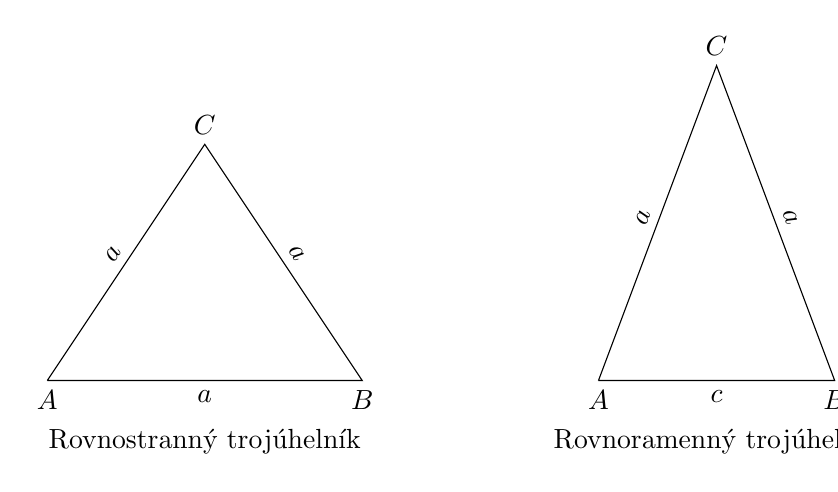
\begin{tikzpicture}
        % rovnostranný trojúhelník
        \draw (-1,0) coordinate (A) node[below] {$A$}
        -- node[midway, below] {$a$}
        (3,0) coordinate (B) node[below] {$B$}
        -- node[midway, above, sloped] {$a$}
        (1,3) coordinate (C) node[above] {$C$}
        -- node[midway, above, sloped] {$a$}
        (A);

        \node[below] at (1, -0.5) {Rovnostranný trojúhelník};

        \hspace{1cm}

        % rovnoramenný trojúhelník
        \draw (5,0) coordinate (D) node[below] {$A$}
        -- node[midway, below] {$c$}
        (8,0) coordinate (E) node[below] {$B$}
        -- node[midway, above, sloped] {$a$}
        (6.5,4) coordinate (F) node[above] {$C$}
        -- node[midway, above, sloped] {$a$}
        (D);

        \node[below] at (6.5,-0.5) {Rovnoramenný trojúhelník};
    \end{tikzpicture}
\end{center}

\subsubsection*{Podle úhlů}

Podle velikosti vnitřních úhlů rozlišujeme \important{ostroúhlý},
\important{tupoúhlý} a \important{pravoúhlý} trojúhelník.

\begin{itemize}
\item \textbf{Ostroúhlý trojúhelník} – všechny jeho vnitřní úhly jsou ostré.
\item \textbf{Tupoúhlý trojúhelník} – jeden jeho vnitřní úhel je tupý.
\item \textbf{Pravoúhlý trojúhelník} – jeden jeho vnitřní úhel je pravý.
\end{itemize}

\begin{center}
    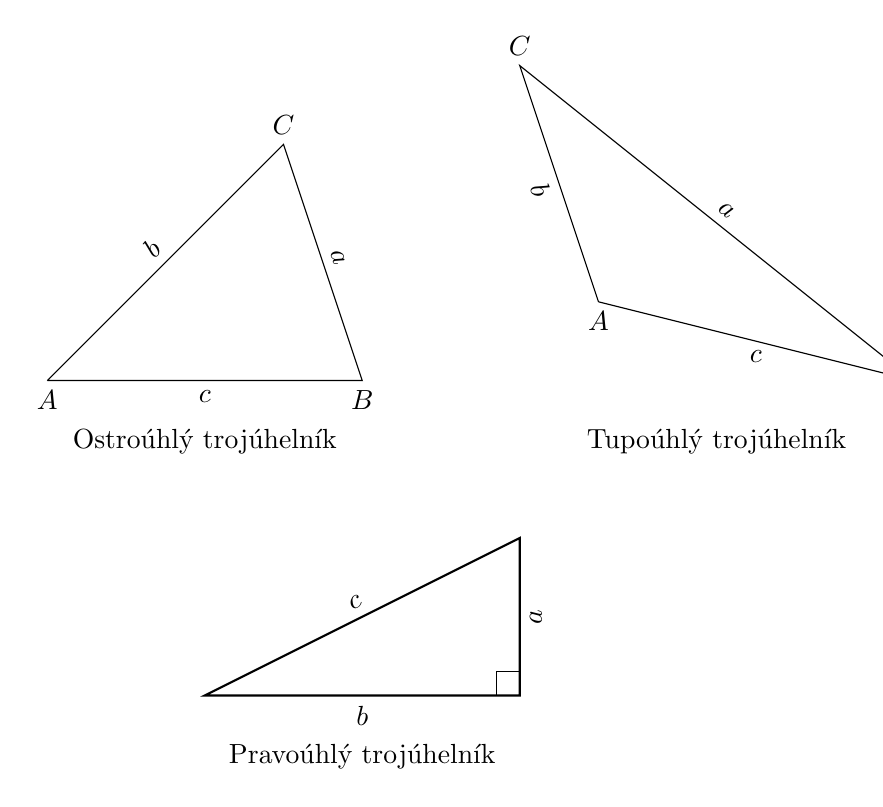
\begin{tikzpicture}
        % ostroúhlý trojúhelník
        \draw (-1,0) coordinate (A) node[below] {$A$}
        -- node[midway, below] {$c$}
        (3,0) coordinate (B) node[below] {$B$}
        -- node[midway, above, sloped] {$a$}
        (2,3) coordinate (C) node[above] {$C$}
        -- node[midway, above, sloped] {$b$}
        (A);

        \node[below] at (1,-0.5) {Ostroúhlý trojúhelník};

        \hspace{1cm}

        % tupoúhlý trojúhelník
        \draw (5,1) coordinate (D) node[below] {$A$}
        -- node[midway, below] {$c$}
        (9,0) coordinate (E) node[below] {$B$}
        -- node[midway, above, sloped] {$a$}
        (4,4) coordinate (F) node[above] {$C$}
        -- node[midway, below, sloped] {$b$}
        (D);

        \node[below] at (6.5,-0.5) {Tupoúhlý trojúhelník};

        
        % pravoúhlý trojúhelník
        \coordinate (A) at (0,-4);
        \coordinate (B) at (4,-4);
        \coordinate (C) at (4,-2);

        \draw[thick] 
        (A) -- node[midway,below] {$b$} 
        (B) -- node[midway,sloped,below] {$a$}
        (C) -- node[midway,sloped,above] {$c$}
        cycle;

        % pravý úhel
        \draw (B) ++(-0.3,0) -- ++(0,0.3) -- ++(0.3,0);

        \node[below] at (2,-4.5) {Pravoúhlý trojúhelník};

    \end{tikzpicture}
\end{center}

Trojúhelník může současně patřit do obou těchto rozdělení.
Například rovnoramenný trojúhelník může být zároveň ostroúhlý,
pravoúhlý nebo tupoúhlý.

\subsection{Vlastnosti trojúhelníku}
Trojúhelník má mnoho zajímavých vlastností a vztahů které v něm lze studovat.
Kromě svých stran a vnitřních úhlů má také další významné prvky, které souvisejí s jeho strukturou a symetrií.

Meti tyto důležité prvky patří například \textbf{výšky}, \textbf{těžnice}, \textbf{střední příčky} a konstrukce různých \textbf{kružnic}
spojených s trojúhelníkem. Tyto prvky často mají společné vlastnosti, například že se jejich
určité přímky protínají v jednom bodě, nebo že vytvářejí významné geometrické vztahy mezi strnami a úhly trojúhelníku.

V následujících kapitolách se budeme podrobněji zabývat těmito prvky a jejich vlastnostmi,
abychom lépe porozuměli komplexní struktuře trojúhelníku a jeho geometrickým vztahům.


\subsubsection*{Výška v trojúhelníku}
V trojúhelníku často potřebujeme zkoumat vztah mezi jeho vrcholy a protilehlými stranami.
Jedním z důležitých prvků, které nám pomáhají tento vztah pochopit, je \textbf{výška trojúhelníku}.

Výška je úsečka, které spojuje vrchol trojúhelníku s protější stranou tak, že je na tuto stranu kolmá.

\begin{definitionbox}
    \textbf{Výška v trojúhelníku} je kolmá úsečka spuštěná z vrcholu trojúhelníku na přímku procházející protější stranou.
\end{definitionbox}

Každý trojúhelník má tři výšky, každou z jednoho vrcholu. Patou výšky nazýváme bod, ve kterém výška protíná přímku procházející protější stranou.

\begin{center}
    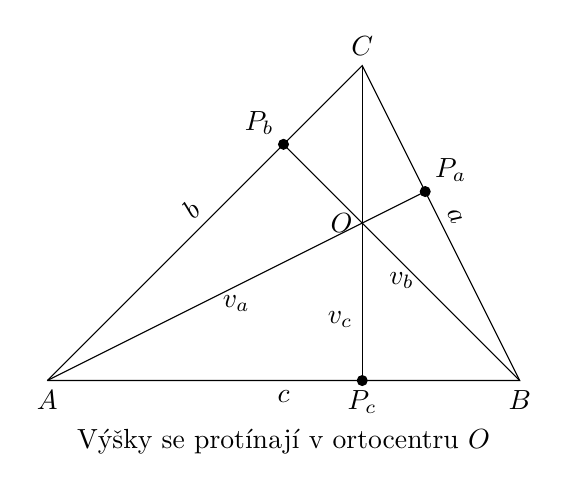
\begin{tikzpicture}
        \draw (0,0) coordinate (A) node[below] {$A$}
        -- node[midway, below] {$c$}
        (6,0) coordinate (B) node[below] {$B$}
        -- node[midway, above, sloped] {$a$}
        (4,4) coordinate (C) node[above] {$C$}
        -- node[midway, above, sloped] {$b$}
        (A);

        % výšky
        \draw (A) -- node[midway, below] {$v_a$} (4.8,2.4);
        \draw (B) -- node[midway, below] {$v_b$} (3,3);
        \draw (C) -- node[near end, below left] {$v_c$} (4,0);

        % paty výšek
        \fill (4.8,2.4) circle (2pt) node[above right] {$P_a$};
        \fill (3,3) circle (2pt) node[above left] {$P_b$};
        \fill (4,0) circle (2pt) node[below] {$P_c$};

        % ortocentrum
        \fill[black] (4,2) circle node[left] {$O$};

        % popisek
        \node [below] at (3,-0.5) {Výšky se protínají v ortocentru $O$};
    \end{tikzpicture}
\end{center}

Výšku z vrcholu $C$ na stranu $AB$ označujeme jako $v_c$. Podobně označujeme i ostatní výšky trojúhelníku.

Zajímavou vlastností výšek je, že všechny tři výšky trojúhenlíku se protínají v jednom bodě. 
Tento bod nazýváme \important{ortocentrum} trojúhelníku a označujeme ho obvykle písmenem $O$.

Toto \textbf{ortocentrum} se nachází uvnitř trojúhelníku, může se však nacházet i mimo něj, v závislosti na typu trojúhelníku.
V ostroúhlém trojúhelníku se ortocentrum nachází uvnitř, v pravoúhlém trojúhelníku se ortocentrum nachází v pravém úhlu, a v tupoúhlém trojúhelníku se ortocentrum nachází mimo trojúhelník.

\begin{center}
    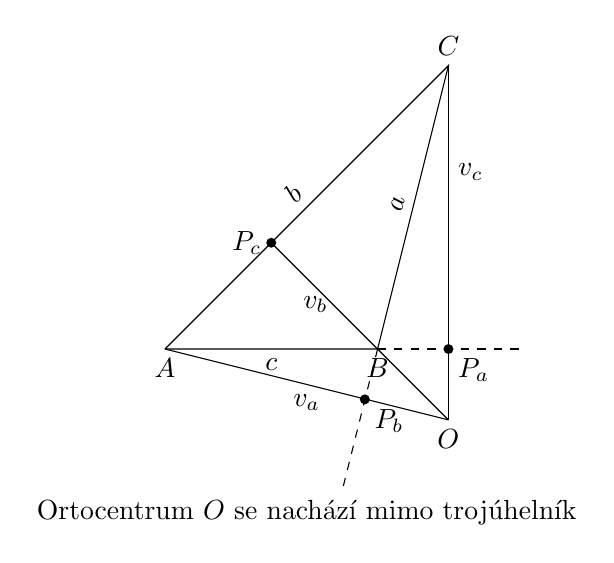
\begin{tikzpicture}[scale=0.9]
        \draw (0,0) coordinate (A) node[below] {$A$}
        -- node[midway, below] {$c$}
        (3,0) coordinate (B) node[below] {$B$}
        -- node[midway, above, sloped] {$a$}
        (4,4) coordinate (C) node[above] {$C$}
        -- node[midway, above, sloped] {$b$}
        (A);

        \draw (4,-1) coordinate (O) node[below] {$O$};

        % výšky
        \draw (A) -- node[midway, below] {$v_a$} (O);
        \draw (1.5,1.5) -- node[near start, below] {$v_b$} (O);
        \draw (C) -- node[near start, below right] {$v_c$} (O);

        % přímky
        \draw[dashed] (B) -- (5,0);
        \draw[dashed] (B) -- (2.5, -2);

        % paty výšek
        \fill (4,0) circle (2pt) node[below right] {$P_a$};
        \fill (2.82,-0.71) circle (2pt) node[below right] {$P_b$};
        \fill (1.5,1.5) circle (2pt) node[left] {$P_c$};

        % popisek
        \node [below] at (2,-2) {Ortocentrum $O$ se nachází mimo trojúhelník};
    \end{tikzpicture}
\end{center}

\begin{notebox}
    Spojením pat výšek trojúhelníku vznikne \textbf{Ortický trojúhelník}.
\end{notebox}

\subsubsection*{Těžnice a těžiště trojúhelníku}

\important{Těžnice} je úsečka, která spojuje vrchol trojúhelníku se středem protější strany.
Pomáhá nám například při studiu symetrie trojúhelníku nebo při určování jeho „středu“.

\begin{definitionbox}
    \textbf{Těžnice} je úsečka, která spojuje vrchol trojúhelníku se středem protější strany.
\end{definitionbox}

Stejně jako u výšek existují v každém trojúhelníku tři těžnice.

\begin{center}
    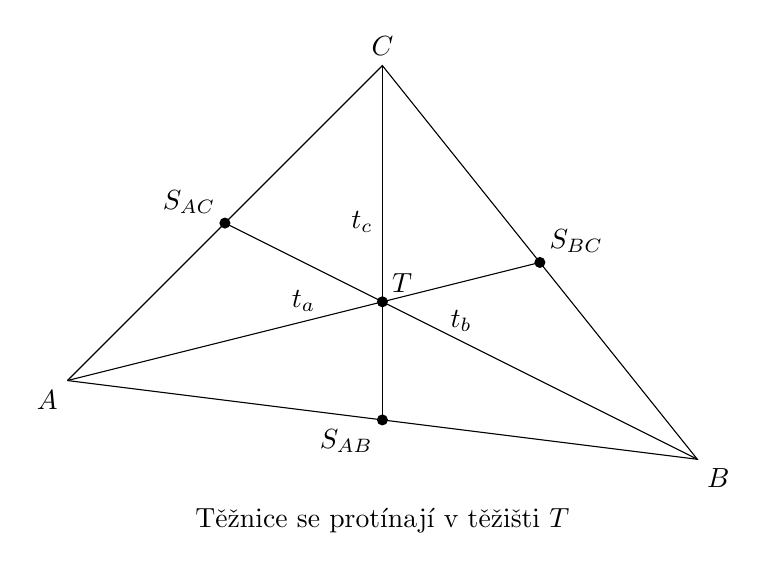
\begin{tikzpicture}
        \draw (0,0) coordinate (A) node[below left] {$A$}
        -- %node[midway, below] {$c$}
        (8,-1) coordinate (B) node[below right] {$B$}
        -- %node[midway, above, sloped] {$a$}
        (4,4) coordinate (C) node[above] {$C$}
        -- %node[midway, above, sloped] {$b$}
        (A);

        % střední příčky
        \fill (4,-0.5) coordinate (SAB) circle (2pt) node[below left] {$S_{AB}$};
        \fill (6,1.5) coordinate (SBC) circle (2pt) node[above right] {$S_{BC}$};
        \fill (2,2) coordinate (SAC) circle (2pt) node[above left] {$S_{AC}$};

        % těžnice
        \draw (C) -- node[midway, above left] {$t_c$} (SAB);
        \draw (A) -- node[midway, above] {$t_a$} (SBC);
        \draw (B) -- node[midway, above] {$t_b$} (SAC);

        % těžiště
        \fill (4,1) coordinate (T) circle (2pt) node[above right] {$T$};
    
        % popisek
        \node [below] at (4,-1.5) {Těžnice se protínají v těžišti $T$};
    \end{tikzpicture}
\end{center}

Těžnice se protínají v jednom bodě, který nazýváme \important{těžiště} trojúhelníku a označujeme ho obvykle písmenem $T$.
Těžiště se nachází uvnitř trojúhelníku a má zajímavou vlastnost, že dělí každou těžnici v poměru 2:1, přičemž delší část těžnice je vždy mezi těžištěm a vrcholem trojúhelníku.

\subsubsection*{Střední příčky}

Středy stran jsme využívali u těžnic, ale můžeme je využít nejen u nich.
Pokud spojíme středy dvou stran trojúhelníku, vznikne nám úsečka, která má zajímavé geometrické vlastnosti.

\begin{definitionbox}
    \textbf{Střední příčka trojúhenlíku} je úsečka, která spojuje středy dvou stran trojúhelníku.
\end{definitionbox}

Každý trojúhelník má tři střední příčky.

\begin{center}
    \begin{tikzpicture}
        \draw (0,0) coordinate (A) node[below left] {$A$}
        -- %node[midway, below] {$c$}
        (8,-1) coordinate (B) node[below right] {$B$}
        -- %node[midway, above, sloped] {$a$}
        (4,4) coordinate (C) node[above] {$C$}
        -- %node[midway, above, sloped] {$b$}
        (A);

        % středy stran
        \fill (4,-0.5) coordinate (SAB) circle (2pt) node[below left] {$S_{AB}$};
        \fill (6,1.5) coordinate (SBC) circle (2pt) node[above right] {$S_{BC}$};
        \fill (2,2) coordinate (SAC) circle (2pt) node[above left] {$S_{AC}$};

        % střední příčky
        \draw (SAB) -- node[midway, below] {$s_c$} (SBC);
        \draw (SBC) -- node[midway, above] {$s_a$} (SAC);
        \draw (SAC) -- node[midway, below] {$s_b$} (SAB);

    \end{tikzpicture}
\end{center}

Střední příčka má dvě důležité vlastnosti:
\begin{itemize}
    \item je \textbf{rovnoběžná} s třetí stranou trojúhelníku,
    \item její délka je \textbf{polovinou} délky třetí strany trojúhelníku.
\end{itemize}

Tyto vlastnosti se někdy shrnují do tzv. \textbf{věty o střední příčce}.


\subsection{Trojúhelníková nerovnost}

Ne každé tři kladné délky mohou tvořit strany trojúhelníku. Jestliže máme trojúhelník $ABC$ se stranami
$a=|BC|$, $b=|CA|$ a $c=|AB|$, musí být každá jeho strana kratší než součet zbývajících dvou stran. Tato
vlastnost vychází z jednoduché geometrické skutečnosti, že nejkratší spojnicí dvou bodů je úsečka, a proto
cesta z jednoho vrcholu do druhého přes třetí vrchol musí být delší než jejich přímé spojení.

\begin{definitionbox}
    Pro délky stran každého trojúhelníku platí \important{trojúhelníkové nerovnosti}
    \[
        a+b>c, \qquad a+c>b, \qquad b+c>a.
    \]
    Trojúhelník s kladnými délkami stran $a$, $b$, $c$ tedy existuje právě tehdy, když jsou splněny všechny tři uvedené nerovnosti.
\end{definitionbox}

Rovnost například $a+b=c$ již trojúhelník nevytváří, protože by všechny tři vrcholy ležely na jedné přímce;
takový útvar označujeme jako \textbf{degenerovaný trojúhelník}. Pokud by dokonce platilo $a+b<c$, nebylo by možné
krajní body strany $c$ spojit dvěma úsečkami délek $a$ a $b$.

Pro praktické úlohy bývá výhodné trojúhelníkové nerovnosti spojit do jednoho vztahu.
Jestliže jsou známy délky dvou stran $a$ a $b$ a hledáme možné hodnoty třetí strany $c$,
vycházíme ze všech tří trojúhelníkových nerovností

\[
    a+b>c,
    \qquad
    a+c>b,
    \qquad
    b+c>a.
\]

První z nich přímo udává horní mez pro délku strany $c$,

\[
    c<a+b.
\]

Z druhé nerovnosti po odečtení $a$ od obou stran dostáváme

\[
    c>b-a,
\]

zatímco ze třetí nerovnosti obdobně plyne

\[
    c>a-b.
\]

Délka strany $c$ tedy musí být větší současně než čísla $a-b$ i $b-a$.
Větší z těchto dvou hodnot je právě absolutní hodnota rozdílu stran $a$ a $b$, protože

\[
    |a-b|
    =
    \begin{cases}
        a-b, & \text{je-li } a\geq b,\\
        b-a, & \text{je-li } a<b.
    \end{cases}
\]

Obě dolní podmínky proto můžeme nahradit jedinou nerovností

\[
    c>|a-b|.
\]

Spojením této dolní meze s horní mezí $c<a+b$ získáme

\[
    |a-b|<c<a+b.
\]

Třetí strana trojúhelníku tedy musí být delší než rozdíl zbývajících dvou stran
a zároveň kratší než jejich součet.

Dolní mez vyjadřuje, že třetí strana musí být delší než rozdíl zbývajících dvou stran, zatímco horní mez říká,
že musí být kratší než jejich součet.

\begin{examplebox}
    Určete, jakých hodnot může nabývat délka třetí strany $c$ trojúhelníku, jestliže $a=3\,\mathrm{cm}$ a $b=5\,\mathrm{cm}$.

    Z trojúhelníkové nerovnosti dostáváme
    \[
        |5-3|<c<5+3,
    \]
    tedy
    \[
        2<c<8.
    \]
    Třetí strana proto může mít libovolnou délku větší než $2\,\mathrm{cm}$ a zároveň menší než $8\,\mathrm{cm}$.
\end{examplebox}



\subsubsection*{Kružnice vepsaná, opsaná a připsaná}

S trojúhelníky dále souvísí několik důležitých kružnic, které jsou určeny stranami a úhly.
Tyto kružnice mají v trojúhelníku zvláštní ostavení a často se využívají při konstrukčních úlohách.

Mezi nejdůležitější kružnice patří \textbf{kružnice opsaná}, \textbf{kružnice vepsaná} a \textbf{kružnice připsaná}.
Každá z těchto kružnic je určena průsečíky určitých přímek v trojúhelníku.

\subsubsection*{Kružnice opsaná}

Kružnice opsaná trojúhelníku je kružnice, která prochází všemi třemi vrcholy trojúhelníku.
Střed této kružnice se nazývá \textbf{střed kružnice opsané} a označuje se obvykle písmenem $S_o$.
Střed kružnice opsané získáme jako průsečík \textbf{os stran trojúhelníku}.

Její poloměr se značí $r$ a je roven vzdálenosti středu kružnice opsané od kterékoli z vrcholů trojúhelníku.

\begin{center}
    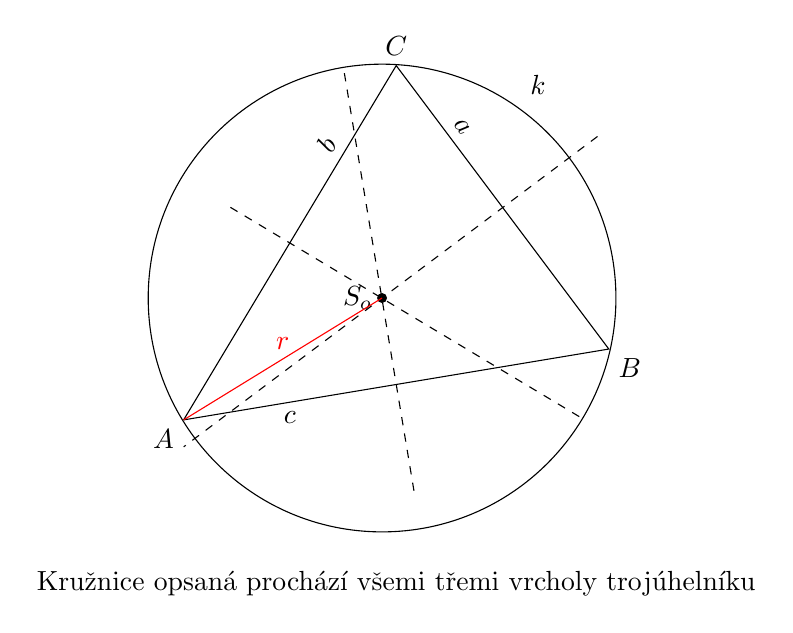
\begin{tikzpicture}[scale=0.9]
        \draw (0,0) coordinate (A) node[below left] {$A$}
        -- node[near start, below] {$c$}
        (6,1) coordinate (B) node[below right] {$B$}
        -- node[near end, above, sloped] {$a$}
        (3,5) coordinate (C) node[above] {$C$}
        -- node[near start, above, sloped] {$b$}
        (A);

        % Body středů stran
        \fill (0.66,3) coordinate (SAC1);
        \fill (5.66,0) coordinate (SAC2);
        \fill (5.84, 4) coordinate (SBC1);
        \fill (0, -0.38) coordinate (SBC2);
        \fill (3.25, -1) coordinate (SAB1);
        \fill (2.25, 5) coordinate (SAB2);

        % osy stran
        \draw[dashed] (SAC1) -- (SAC2);
        \draw[dashed] (SBC1) -- (SBC2);
        \draw[dashed] (SAB1) -- (SAB2);

        % střed kružnice opsané
        \fill (2.8,1.72) coordinate (So) circle (2pt) node[left] {$S_o$};

        % kružnice opsaná
        \draw (So) circle (3.3);

        % poloměr
        \draw[-,red] (So) -- node[above] {$r$} (A);
            
        % popisek kružnice
        \node [below] at (3,-2) {Kružnice opsaná prochází všemi třemi vrcholy trojúhelníku};
        \node [below] at (5,5) {$k$};

    \end{tikzpicture}
\end{center}

\subsubsection*{Kružnice vepsaná}
Kružnice vepsaná trojúhelníku je kružnice, která se dotýká právě jednou každé ze tří stran trojúhelníku.
Střed této kružnice se nazývá \textbf{střed kružnice vepsané} a označuje se obvykle písmenem $S_v$.
Střed kružnice vepsané získáme jako průsečík \textbf{os vnitřních úhlů trojúhelníku}.
Její poloměr se značí $\rho$ a je rovne vzdálenosti úsečky, vedené ze středu kolmo na stranu, od které se dotýká.

\begin{center}
    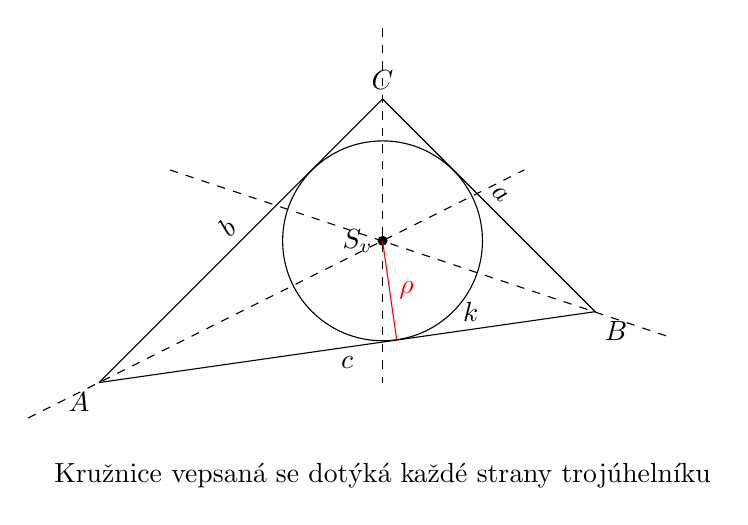
\begin{tikzpicture}[scale=0.9]
        \draw (0,0) coordinate (A) node[below left] {$A$}
        -- node[midway, below] {$c$}
        (7,1) coordinate (B) node[below right] {$B$}
        -- node[midway, above, sloped] {$a$}
        (4,4) coordinate (C) node[above] {$C$}
        -- node[midway, above, sloped] {$b$}
        (A);

        % body os úhlů
        \fill (-1,-0.5) coordinate (OA1);
        \fill (6,3) coordinate (OA2);
        \fill (8,0.66) coordinate (OB1);
        \fill (1,3) coordinate (OB2);
        \fill (4,5) coordinate (OC1);
        \fill (4,0) coordinate (OC2);

        % osy vnitřních úhlů
        \draw[dashed] (OA1) -- (OA2);
        \draw[dashed] (OB1) -- (OB2);
        \draw[dashed] (OC1) -- (OC2);

        % střed kružnice vepsané
        \fill (4,2) coordinate (Sv) circle (2pt) node[left] {$S_v$};

        % kružnice vepsaná
        \draw (Sv) circle (1.41);

        % poloměr
        \fill (4.2,0.6) coordinate (P);
        \draw[-,red] (Sv) -- node[right] {$\rho$} (P);

        % popisek kružnice
        \node [below] at (4,-1) {Kružnice vepsaná se dotýká každé strany trojúhelníku};
        \node [right] at (5,1) {$k$};

    \end{tikzpicture}
\end{center}


\subsubsection*{Kružnice připsané}

Kromě kruznice vepsané existují také tzv. \textbf{krunžnice připsané}, 
které se dotýkají jedné strany trojúhelníku a prodloužení zbývajících dvou stran.

Každý trojúhelník má třit takové kružnice připsané,
protože každé straně odpovídá jedan taková kružnice.

Středy těchto kružnic získáme jako průsečíky \textbf{os vnitřních a vnějších úhlů trojúhelníku}.
Poloměry krunžnic připsaných se značí $\rho_a$, $\rho_b$ a $\rho_c$ a jsou rovny vzdálenosti úsečky, vedené ze středu kolmo na stranu, od které se dotýká, od které se dotýká.
Všechny tyto poloměry jsou si rovny, jen v případě, že se jedná o rovnostranný trojúhelník.

\begin{center}
    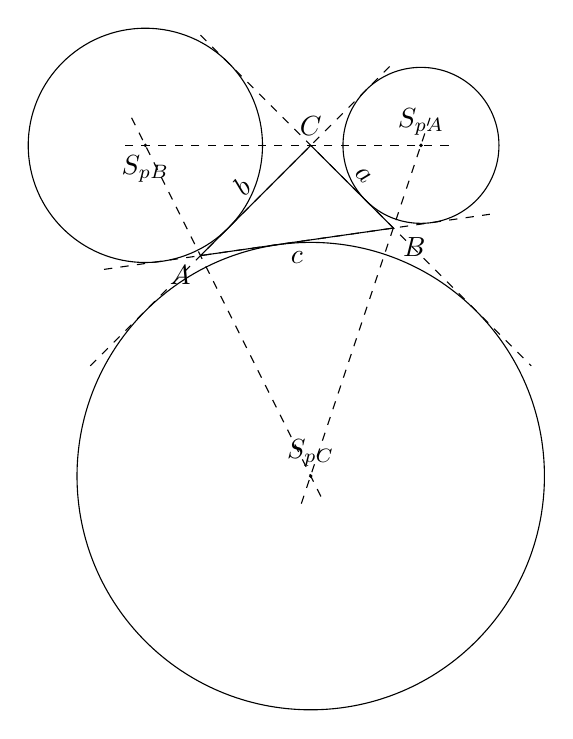
\begin{tikzpicture}[scale=0.35]
        \draw (0,0) coordinate (A) node[below left] {$A$}
        -- node[midway, below] {$c$}
        (7,1) coordinate (B) node[below right] {$B$}
        -- node[midway, above, sloped] {$a$}
        (4,4) coordinate (C) node[above] {$C$}
        -- node[midway, above, sloped] {$b$}
        (A);

        % body os úhlů
        \fill (-2.5,5) coordinate (OA1);
        \fill (4.5,-9) coordinate (OA2);
        \fill (3.66,-9) coordinate (OB1);
        \fill (8.33, 5) coordinate (OB2);
        \fill (9,4) coordinate (OC1);
        \fill (-3,4) coordinate (OC2);

        % přímky prodloužení stran
        \draw[dashed] (0,8) -- (12,-4);
        \draw[dashed] (-4,-4) -- (7,7);
        \draw[dashed] (-3.5,-0.5) -- (10.5,1.5);

        % osy vnitřních a vnějších úhlů
        \draw[dashed] (OA1) -- (OA2);
        \draw[dashed] (OB1) -- (OB2);
        \draw[dashed] (OC1) -- (OC2);

        % středy kružnic připsaných
        \fill (8,4) coordinate (SpA) circle (2pt) node[above] {$S_{pA}$};
        \fill (-2,4) coordinate (SpB) circle (2pt) node[below] {$S_{pB}$};
        \fill (4,-8) coordinate (SpC) circle (2pt) node[above] {$S_{pC}$};

        % kružnice připsané
        \draw (SpA) circle (2.83);
        \draw (SpB) circle (4.25);
        \draw (SpC) circle (8.48);


    \end{tikzpicture}
\end{center}

\section{Mnohoúhelník}

Dosud jsme se zabývali převážně trojúhelníky. Ty však jsou nejjednodušším případem
obecnějšího geometrického útvaru, kterým jsou \textbf{mnohoúhelníky}.

\begin{definitionbox}
    \textbf{Mnohoúhelník} je rovinný geometrický útvar, který vznikne průnikem konečného počtu polorovin, jejichž hranice tvoří uzavřenou lomenou čáru.
\end{definitionbox}

Body, ve kterých se jednotlivé úsečky setkávají, nazýváme \textbf{vrcholy mnohoúhelníku}.
Úsečky spojující sousední body jsou pak \textbf{stranami mnohoúhelníku}.
Mnohoúhelníky můžeme rozlišit například podle počtu stran, přičemž nejběžnější jsou čtyřúhelníky, pětiúhelníky a šestiúhelníky a poté obecně $n$-úhelníky.

\begin{center}
    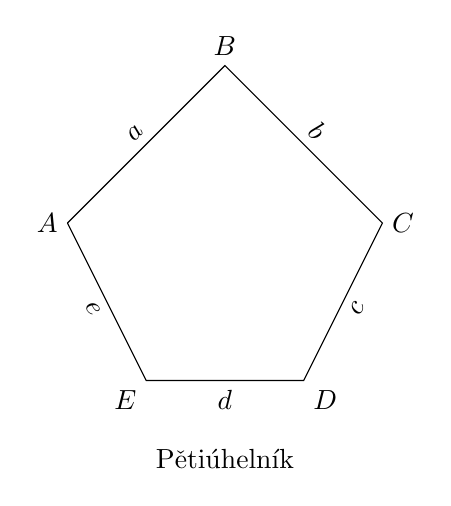
\begin{tikzpicture}
        % mnohoúhelník
        \draw (0,0) coordinate (A) node[left] {$A$}
        -- node[midway, above, sloped] {$a$}
        (2,2) coordinate (B) node[above] {$B$}
        -- node[midway, above, sloped] {$b$}
        (4,0) coordinate (C) node[right] {$C$}
        -- node[midway, below, sloped] {$c$}
        (3,-2) coordinate (D) node[below right] {$D$}
        -- node[midway, below, sloped] {$d$}
        (1,-2) coordinate (E) node[below left] {$E$}
        -- node[midway, below, sloped] {$e$}
        (A);

        \node at (2,-3) {Pětiúhelník};

    \end{tikzpicture}
\end{center}

\subsection{Úhlopříčky mnohoúhelníku}

\important{Úhlopříčka} je úsečka, která spojuje dva nesousední vrcholy mnohoúhelníku.
Každý mnohoúhelník má $\frac{1}{2}n(n-3)$ úhlopříček, kde $n$ je počet vrcholů mnohoúhelníku.

\begin{center}
    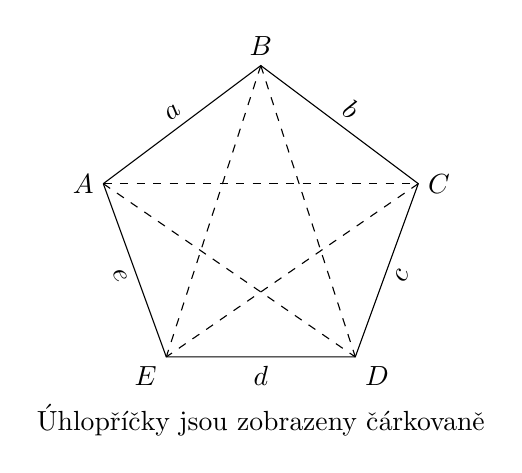
\begin{tikzpicture}
        % mnohoúhelník
        \draw (0,0) coordinate (A) node[left] {$A$}
        -- node[midway, above, sloped] {$a$}
        (2,1.5) coordinate (B) node[above] {$B$}
        -- node[midway, above, sloped] {$b$}
        (4,0) coordinate (C) node[right] {$C$}
        -- node[midway, below, sloped] {$c$}
        (3.2,-2.2) coordinate (D) node[below right] {$D$}
        -- node[midway, below, sloped] {$d$}
        (0.8,-2.2) coordinate (E) node[below left] {$E$}
        -- node[midway, below, sloped] {$e$}
        (A);

        % úhlopříčky
        \draw[dashed] (A) -- (C);
        \draw[dashed] (A) -- (D);
        \draw[dashed] (B) -- (D);
        \draw[dashed] (B) -- (E);
        \draw[dashed] (C) -- (E);
    
        % popisek
        \node at (2,-3) {Úhlopříčky jsou zobrazeny čárkovaně};
    \end{tikzpicture}
\end{center}

\subsection{Součet vnitřních úhlů mnohoúhelníku}
Součet vnitřních úhlů mnohoúhelníku s $n$ stranami je dán vzorcem $(n-2) \cdot 180°$.
Tento vzorec lze odvodit například rozdělením mnohoúhelníku na $n-2$ trojúhelníků, přičemž každý z nich má součet vnitřních úhlů 180°.




\subsection{Konvexní a nekonvexní mnohoúhelník}
Mnohoúhelníky můžeme rozdělit do dvou základních skupin podle toho, zda obsahují vnitřní úhly větší než 180°.

\begin{definitionbox}
    \textbf{Konvexní mnohoúhelník} je mnohoúhelník, který nemá žádný vnitřní úhel větší než 180°.
\end{definitionbox}

\begin{definitionbox}
    \textbf{Nekonvexní mnohoúhelník} je mnohoúhelník, který má alespoň jeden vnitřní úhel větší než 180°.
\end{definitionbox}


\begin{center}
    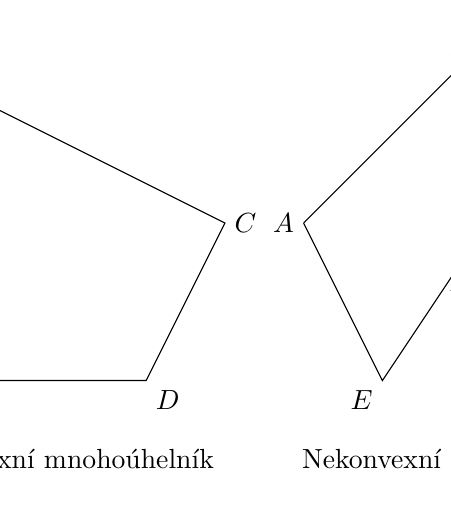
\begin{tikzpicture}
        \hspace{-2cm}
        % konvexní mnohoúhelník
        \draw (0,0) coordinate (A) node[left] {$A$}
        -- (1,1.5) coordinate (B) node[above] {$B$}
        -- (4,0) coordinate (C) node[right] {$C$}
        -- (3,-2) coordinate (D) node[below right] {$D$}
        -- (1,-2) coordinate (E) node[below left] {$E$}
        -- (-0.2,-1) coordinate (F) node[below] {$F$}
        -- (A);

        \node at (2,-3) {Konvexní mnohoúhelník};
        \hspace{5cm}
        % nekonvexní mnohoúhelník
        \draw (0,0) coordinate (A) node[left] {$A$}
        -- (2,2) coordinate (B) node[above] {$B$}
        -- (4,0) coordinate (C) node[right] {$C$}
        -- (2,-0.5) coordinate (D) node[below] {$D$}
        -- (1,-2) coordinate (E) node[below left] {$E$}
        -- (A);

        \node at (2,-3) {Nekonvexní mnohoúhelník};
    \end{tikzpicture}
\end{center}

\subsection{Pravidelné mnohoúhelníky}
Zvláštním případem mnohoúhelníku jsou \important{pravidelné mnohoúhelníky}, které mají všechny strany stejně dlouhé a všechny vnitřní úhly stejně velké.

Mezi pravidelné mnohoúhelníky patří například rovnostranný trojúhelník, čtverec, pravidelný pětiúhelník a další.

\begin{center}
    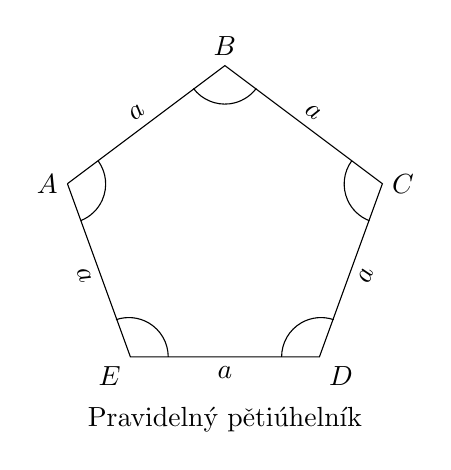
\begin{tikzpicture}
        % pravidelný pětiúhelník
        \draw (0,0) coordinate (A) node[left] {$A$}
        -- node[midway, above, sloped] {$a$}
        (2,1.5) coordinate (B) node[above] {$B$}
        -- node[midway, above, sloped] {$a$}
        (4,0) coordinate (C) node[right] {$C$}
        -- node[midway, below, sloped] {$a$}
        (3.2,-2.2) coordinate (D) node[below right] {$D$}
        -- node[midway, below, sloped] {$a$}
        (0.8,-2.2) coordinate (E) node[below left] {$E$}
        -- node[midway, below, sloped] {$a$}
        (A);

        % úhly
        \draw (A) ++(0.39,0.29) arc (36:-68:0.5);
        \draw (B) ++(-0.40,-0.29) arc (-143:-37:0.5);
        \draw (C) ++(-0.39,0.29) arc (144:249:0.5);
        \draw (D) ++(-0.48,0) arc (180:71:0.5);
        \draw (E) ++(0.48,0) arc (0:109:0.5);

        \node at (2,-3) {Pravidelný pětiúhelník};
    \end{tikzpicture}
\end{center}



\subsection{Rozdělení čtyřúhelníků}

Čtyřúhelníky tvoří velmi rozmanitou skupinu rovinných útvarů. Některé z nich rozlišujeme
podle rovnoběžnosti stran, jiné podle jejich délek, velikostí úhlů nebo podle zvláštních
vlastností jejich úhlopříček. Abychom se v této množině útvarů dobře orientovali, je vhodné
si ukázat jejich základní rozdělení a zároveň zdůraznit, jaké vlastnosti jsou pro jednotlivé
typy čtyřúhelníků charakteristické.

Nejprve připomeňme, že každý čtyřúhelník je rovinný útvar tvořený čtyřmi vrcholy a čtyřmi
stranami. Součet jeho vnitřních úhlů je vždy roven
\[
    360^\circ.
\]

\begin{notebox}
V následujícím přehledu budeme používat \textbf{inkluzivní definici lichoběžníku}, tedy že
\important{lichoběžník je čtyřúhelník, který má alespoň jednu dvojici protějších stran rovnoběžných}.
Díky tomu je každý rovnoběžník zároveň zvláštním případem lichoběžníku.
Pokud bys chtěl používat výlučnou definici, stačí tuto část snadno upravit.
\end{notebox}


\subsubsection{Základní rozdělení}

\begin{figure}[ht]
    \centering
    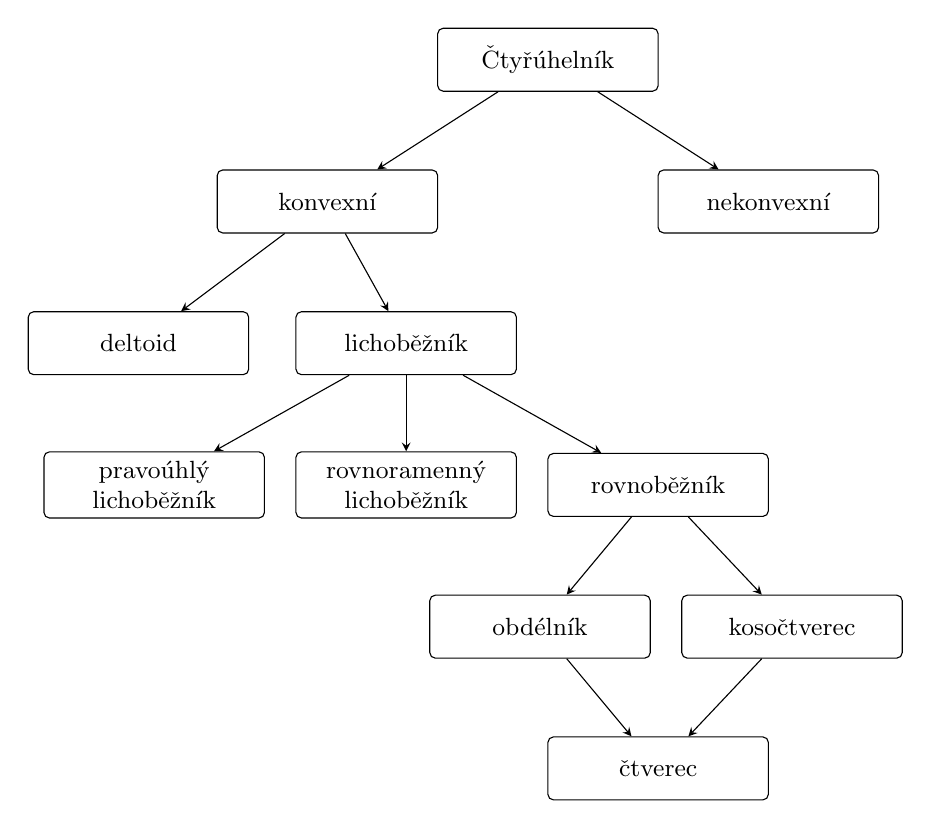
\begin{tikzpicture}[
        every node/.style={
            draw,
            rounded corners=2pt,
            minimum width=28mm,
            minimum height=8mm,
            align=center,
            font=\small
        },
        line/.style={->, >=stealth, thin}
    ]

        % 1. úroveň
        \node (ctyr) at (0,0) {Čtyřúhelník};

        % 2. úroveň
        \node (konv) at (-2.8,-1.8) {konvexní};
        \node (nekonv) at (2.8,-1.8) {nekonvexní};

        % 3. úroveň
        \node (deltoid) at (-5.2,-3.6) {deltoid};
        \node (lich) at (-1.8,-3.6) {lichoběžník};

        % 4. úroveň
        \node (pravlich) at (-5,-5.4) {pravoúhlý\\ lichoběžník};
        \node (rovnlich) at (-1.8,-5.4) {rovnoramenný\\ lichoběžník};
        \node (rovnob) at (1.4,-5.4) {rovnoběžník};

        % 5. úroveň
        \node (obd) at (-0.1,-7.2) {obdélník};
        \node (kos) at (3.1,-7.2) {kosočtverec};

        % 6. úroveň
        \node (ctv) at (1.4,-9.0) {čtverec};

        % spojnice
        \draw[line] (ctyr) -- (konv);
        \draw[line] (ctyr) -- (nekonv);

        \draw[line] (konv) -- (deltoid);
        \draw[line] (konv) -- (lich);

        \draw[line] (lich) -- (pravlich);
        \draw[line] (lich) -- (rovnlich);
        \draw[line] (lich) -- (rovnob);

        \draw[line] (rovnob) -- (obd);
        \draw[line] (rovnob) -- (kos);

        \draw[line] (obd) -- (ctv);
        \draw[line] (kos) -- (ctv);

    \end{tikzpicture}
    \caption{Základní vztahy mezi vybranými typy čtyřúhelníků.}
    \label{fig:quadrilateral_classification}
\end{figure}
Z předchozího schématu je vidět základní hierarchie čtyřúhelníků. Zvláštní pozornost si
zaslouží útvar \textbf{čtverec}, protože jej lze chápat dvojím způsobem: je to současně
\textbf{obdélník se všemi stranami shodnými} a zároveň \textbf{kosočtverec se všemi úhly pravými}.
Čtverec tedy dědí vlastnosti obdélníku i kosočtverce zároveň.

\subsubsection{Konvexní a nekonvexní čtyřúhelník}

\begin{definitionbox}
Čtyřúhelník nazýváme \textbf{konvexní}, jestliže celá úsečka spojující libovolné dva jeho body
leží uvnitř čtyřúhelníku nebo na jeho hranici.

Čtyřúhelník nazýváme \textbf{nekonvexní} (nebo také \textbf{konkávní}), jestliže tato vlastnost
neplatí.
\end{definitionbox}

U konvexního čtyřúhelníku leží všechny vnitřní úhly menší než $180^\circ$, zatímco
u nekonvexního čtyřúhelníku je alespoň jeden vnitřní úhel větší než $180^\circ$.

\subsubsection{Deltoid}

\begin{definitionbox}
\important{Deltoid} je čtyřúhelník, který má dvě dvojice shodných sousedních stran.
\end{definitionbox}

Je-li $ABCD$ deltoid a platí například
\[
    |AB|=|AD|,
    \qquad
    |BC|=|CD|,
\]
pak pro něj platí tyto důležité vlastnosti:

\begin{itemize}
    \item jedna úhlopříčka je osou souměrnosti deltoidu,
    \item úhlopříčky jsou na sebe kolmé,
    \item hlavní úhlopříčka půlí druhou úhlopříčku,
    \item hlavní úhlopříčka zároveň půlí dvojici protilehlých úhlů.
\end{itemize}

\subsubsection{Lichoběžník}

\begin{definitionbox}
\important{Lichoběžník} je čtyřúhelník, který má alespoň jednu dvojici protějších stran rovnoběžných.
Rovnoběžné strany nazýváme \textbf{základny}, zbývající dvě strany nazýváme \textbf{ramena}.
\end{definitionbox}

K lichoběžníku se váže několik základních pojmů a vlastností:

\begin{itemize}
    \item vzdálenost základen nazýváme \textbf{výška lichoběžníku},
    \item spojnice středů ramen se nazývá \textbf{střední příčka lichoběžníku},
    \item pro délku střední příčky platí
    \[
        s = \frac{a+c}{2},
    \]
    kde $a$, $c$ jsou délky obou základen.
\end{itemize}

\paragraph{Pravoúhlý lichoběžník.}
Pravoúhlý lichoběžník je takový lichoběžník, který má jeden vnitřní úhel pravý.
Protože sousední úhly při rameni jsou vedlejší, má ve skutečnosti pravé úhly dva.

\paragraph{Rovnoramenný lichoběžník.}
Rovnoramenný lichoběžník je takový lichoběžník, jehož ramena mají stejnou délku.
Pro rovnoramenný lichoběžník dále platí:

\begin{itemize}
    \item úhly při jedné základně jsou shodné,
    \item úhly při druhé základně jsou rovněž shodné,
    \item úhlopříčky mají stejnou délku.
\end{itemize}

\subsubsection{Rovnoběžník}

\begin{definitionbox}
\important{Rovnoběžník} je čtyřúhelník, jehož obě dvojice protějších stran jsou rovnoběžné.
\end{definitionbox}

Pro rovnoběžník platí řada důležitých vlastností, které z něj činí jeden ze základních
útvarů planimetrie:

\begin{itemize}
    \item protější strany jsou rovnoběžné a zároveň shodné,
    \item protější úhly jsou shodné,
    \item sousední úhly jsou vedlejší, a jejich součet je tedy $180^\circ$,
    \item úhlopříčky se navzájem půlí.
\end{itemize}

\subsubsection{Obdélník}

\begin{definitionbox}
\important{Obdélník} je rovnoběžník, který má alespoň jeden pravý úhel.
\end{definitionbox}

Protože v rovnoběžníku jsou sousední úhly vedlejší a protější úhly shodné, plyne z této
definice, že obdélník má ve skutečnosti \textbf{všechny čtyři úhly pravé}. Dále pro něj platí:

\begin{itemize}
    \item protější strany jsou rovnoběžné a shodné,
    \item všechny vnitřní úhly mají velikost $90^\circ$,
    \item úhlopříčky se navzájem půlí,
    \item úhlopříčky mají stejnou délku.
\end{itemize}

\subsubsection{Kosočtverec}

\begin{definitionbox}
\important{Kosočtverec} je rovnoběžník, jehož všechny čtyři strany mají stejnou délku.
\end{definitionbox}

Z toho okamžitě plyne, že kosočtverec je zároveň zvláštním případem rovnoběžníku,
a dědí tedy všechny jeho vlastnosti. Kromě toho pro něj ještě navíc platí:

\begin{itemize}
    \item všechny strany jsou shodné,
    \item úhlopříčky se navzájem půlí,
    \item úhlopříčky jsou na sebe kolmé,
    \item každá úhlopříčka půlí dvojici protilehlých úhlů.
\end{itemize}

\subsubsection{Čtverec}

\begin{definitionbox}
\important{Čtverec} je čtyřúhelník, který má všechny strany stejně dlouhé a všechny vnitřní úhly pravé.
\end{definitionbox}

Čtverec je tedy zároveň \textbf{obdélníkem} i \textbf{kosočtvercem}, a proto sdružuje jejich
vlastnosti. Platí pro něj zejména:

\begin{itemize}
    \item všechny strany jsou shodné,
    \item všechny vnitřní úhly mají velikost $90^\circ$,
    \item protější strany jsou rovnoběžné,
    \item úhlopříčky mají stejnou délku,
    \item úhlopříčky se navzájem půlí,
    \item úhlopříčky jsou na sebe kolmé,
    \item každá úhlopříčka půlí dvojici protilehlých úhlů.
\end{itemize}

\subsubsection{Shrnutí vztahů mezi základními typy čtyřúhelníků}

Z hlediska zařazení jednotlivých útvarů je užitečné si pamatovat následující vztahy:

\begin{itemize}
    \item každý obdélník je rovnoběžník,
    \item každý kosočtverec je rovnoběžník,
    \item každý rovnoběžník je při zvolené definici zároveň lichoběžník,
    \item každý čtverec je současně obdélník i kosočtverec,
    \item ne každý lichoběžník je rovnoběžník,
    \item ne každý deltoid je kosočtverec.
\end{itemize}

\begin{notebox}
Později, až budeme probírat kružnice, můžeme k tomuto přehledu doplnit ještě další
zajímavé typy čtyřúhelníků, například \textbf{tětivový čtyřúhelník} (tedy čtyřúhelník
vepsaný do kružnice) nebo \textbf{tečnový čtyřúhelník} (tedy čtyřúhelník opsaný kružnici).
Tyto útvary mají další specifické vlastnosti, ale pro první přehled základních typů
čtyřúhelníků není nutné je zavádět hned.
\end{notebox}


% ------------------------------------------------------------
% NOVÁ SEKCE ZA ČTYŘÚHELNÍKY
% ------------------------------------------------------------

\section{Kružnice a kruh}

Kružnice a kruh patří mezi základní rovinné geometrické útvary. Přestože se jejich názvy v běžném jazyce někdy zaměňují,
v geometrii označují dva různé objekty: kružnice tvoří pouze hranici, zatímco kruh obsahuje tuto hranici i všechny body
uvnitř ní. Oba útvary přitom určujeme pomocí jednoho bodu, který nazýváme střed, a jednoho kladného čísla, které udává poloměr.

\subsection{Kružnice}

\begin{definitionbox}
    Nechť je dán bod $S$ a kladné reálné číslo $r$. \important{Kružnice} se středem $S$ a poloměrem $r$ je množina
    všech bodů roviny, jejichž vzdálenost od bodu $S$ je právě $r$:
    \[
        k(S;r)=\{X\mid |SX|=r\}.
    \]
\end{definitionbox}

Bod $S$ nazýváme \textbf{střed kružnice} a číslo $r$ jejím \textbf{poloměrem}. Slovem poloměr přitom podle kontextu
označujeme nejen číslo $r$, ale také libovolnou úsečku, která spojuje střed kružnice s některým jejím bodem.

\subsection{Kruh}

\begin{definitionbox}
    Nechť je dán bod $S$ a kladné reálné číslo $r$. \important{Kruh} se středem $S$ a poloměrem $r$ je množina
    všech bodů roviny, jejichž vzdálenost od bodu $S$ je menší nebo rovna $r$:
    \[
        K(S;r)=\{X\mid |SX|\leq r\}.
    \]
\end{definitionbox}

Kružnice $k(S;r)$ tvoří hranici kruhu $K(S;r)$. Body, jejichž vzdálenost od středu je menší než $r$, tvoří
\textbf{vnitřek kruhu}, zatímco body ve vzdálenosti větší než $r$ leží vně kruhu.

\begin{center}
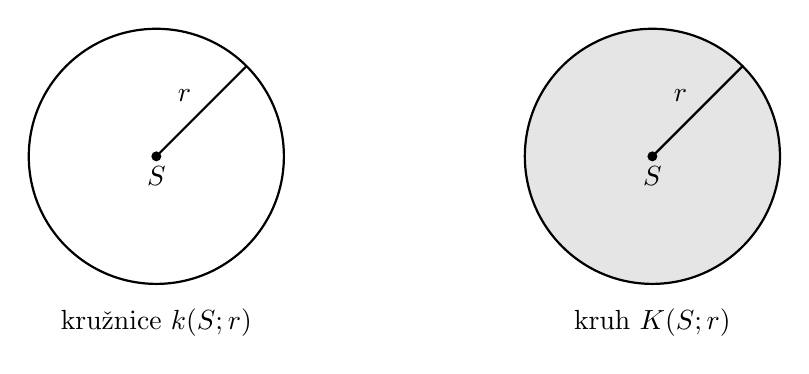
\begin{tikzpicture}[scale=0.9]
    % kružnice
    \begin{scope}[shift={(-3.5,0)}]
        \draw[thick] (0,0) circle (1.8);
        \fill (0,0) circle (2pt) node[below] {$S$};
        \draw[thick] (0,0)--(1.27,1.27) node[midway, above left] {$r$};
        \node at (0,-2.35) {kružnice $k(S;r)$};
    \end{scope}

    % kruh
    \begin{scope}[shift={(3.5,0)}]
        \filldraw[fill=gray!20, draw=black, thick] (0,0) circle (1.8);
        \fill (0,0) circle (2pt) node[below] {$S$};
        \draw[thick] (0,0)--(1.27,1.27) node[midway, above left] {$r$};
        \node at (0,-2.35) {kruh $K(S;r)$};
    \end{scope}
\end{tikzpicture}
\end{center}

\subsection{Tětiva a průměr}

Zvolíme-li na kružnici dva různé body $A$ a $B$, můžeme je spojit úsečkou. Taková úsečka se nazývá tětiva.

\begin{definitionbox}
    \important{Tětiva kružnice} je úsečka, jejíž oba krajní body leží na kružnici.
\end{definitionbox}

Prochází-li tětiva středem kružnice, nazýváme ji \important{průměr}. Jeho délku značíme $d$ a vždy platí
\[
    d=2r.
\]
Průměr je zároveň nejdelší možnou tětivou dané kružnice.

\begin{center}
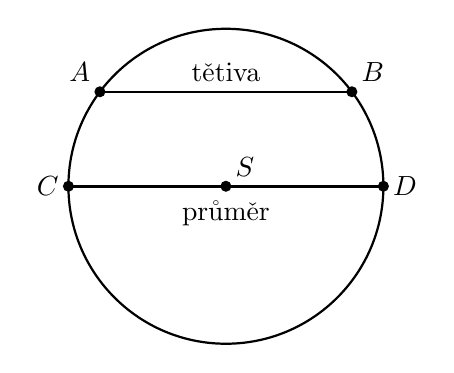
\begin{tikzpicture}[scale=1]
    \draw[thick] (0,0) circle (2);
    \fill (0,0) circle (2pt) node[above right] {$S$};

    \coordinate (A) at (-1.6,1.2);
    \coordinate (B) at (1.6,1.2);
    \draw[thick] (A)--(B);
    \fill (A) circle (2pt) node[above left] {$A$};
    \fill (B) circle (2pt) node[above right] {$B$};
    \node at (0,1.45) {tětiva};

    \coordinate (C) at (-2,0);
    \coordinate (D) at (2,0);
    \draw[very thick] (C)--(D);
    \fill (C) circle (2pt) node[left] {$C$};
    \fill (D) circle (2pt) node[right] {$D$};
    \node at (0,-0.35) {průměr};
\end{tikzpicture}
\end{center}

\subsection{Kružnicový oblouk}

Dva různé body $A$ a $B$ na kružnici rozdělují kružnici na dvě části, které nazýváme \important{kružnicové oblouky}.
Body $A$ a $B$ jsou jejich společnými krajními body. Pokud úsečka $AB$ není průměrem, rozlišujeme \textbf{menší oblouk}
a \textbf{větší oblouk} $AB$; jestliže je $AB$ průměrem, vznikají dvě stejně velké části kružnice, které nazýváme
\textbf{půlkružnice}.

\subsection{Kruhová výseč a kruhová úseč}

Dva poloměry $SA$ a $SB$ spolu s příslušným obloukem kružnice vymezují část kruhu, kterou nazýváme kruhová výseč.
Naopak tětiva $AB$ spolu s příslušným obloukem vymezuje kruhovou úseč.

\begin{definitionbox}
    \important{Kruhová výseč} je část kruhu ohraničená dvěma poloměry a obloukem kružnice.

    \medskip

    \important{Kruhová úseč} je část kruhu ohraničená tětivou a příslušným obloukem kružnice.
\end{definitionbox}

\begin{center}
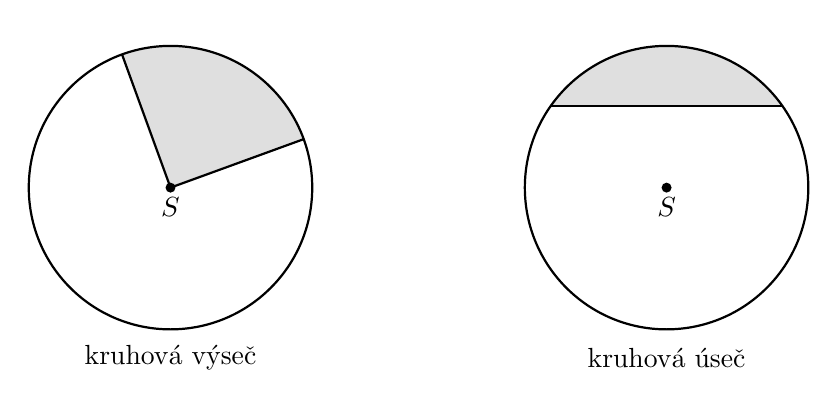
\begin{tikzpicture}[scale=0.9]
    % výseč
    \begin{scope}[shift={(-3.5,0)}]
        \fill[gray!25] (0,0)--(20:2) arc (20:110:2)--cycle;
        \draw[thick] (0,0) circle (2);
        \draw[thick] (0,0)--(20:2) (0,0)--(110:2);
        \fill (0,0) circle (2pt) node[below] {$S$};
        \node at (0,-2.4) {kruhová výseč};
    \end{scope}

    % úseč
    \begin{scope}[shift={(3.5,0)}]
        \fill[gray!25] (35:2) arc (35:145:2)--cycle;
        \draw[thick] (0,0) circle (2);
        \draw[thick] (35:2)--(145:2);
        \fill (0,0) circle (2pt) node[below] {$S$};
        \node at (0,-2.4) {kruhová úseč};
    \end{scope}
\end{tikzpicture}
\end{center}

Je-li tětiva průměrem kružnice, rozděluje kruh na dva \textbf{půlkruhy}.

\subsection{Vzájemná poloha přímky a kružnice}

Vzájemnou polohu přímky $p$ a kružnice $k(S;r)$ můžeme určit podle počtu jejich společných bodů. Stejnou situaci lze
popsat také pomocí vzdálenosti středu kružnice od přímky; označme tuto vzdálenost $v=d(S,p)$.

\begin{definitionbox}
    Pro přímku $p$ a kružnici $k(S;r)$ nastává právě jedna z následujících možností:
    \[
    \begin{array}{c|c|c}
        \text{poloha přímky} & \text{počet společných bodů} & \text{podmínka} \\
        \hline
        \text{sečna} & 2 & v<r \\
        \text{tečna} & 1 & v=r \\
        \text{vnější přímka} & 0 & v>r
    \end{array}
    \]
\end{definitionbox}

\begin{center}
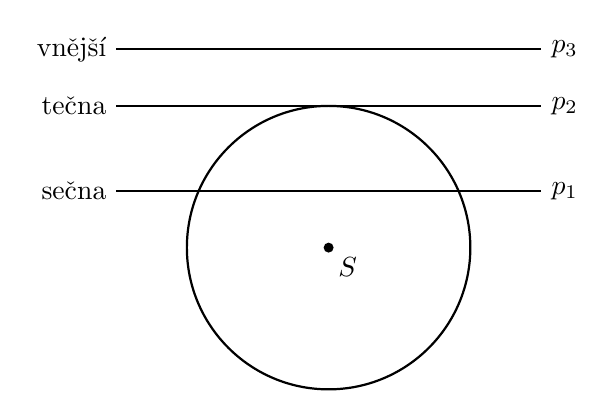
\begin{tikzpicture}[scale=0.9]
    \draw[thick] (0,0) circle (2);
    \fill (0,0) circle (2pt) node[below right] {$S$};

    \draw[thick] (-3,0.8)--(3,0.8) node[right] {$p_1$};
    \draw[thick] (-3,2)--(3,2) node[right] {$p_2$};
    \draw[thick] (-3,2.8)--(3,2.8) node[right] {$p_3$};

    \node[left] at (-3,0.8) {sečna};
    \node[left] at (-3,2) {tečna};
    \node[left] at (-3,2.8) {vnější};
\end{tikzpicture}
\end{center}

Pokud je přímka sečnou kružnice a protíná ji v bodech $A$ a $B$, vzniká tětiva $AB$. Kolmice vedená ze středu kružnice
na tuto tětivu ji půlí, a proto je pata této kolmice středem úsečky $AB$.

\begin{notebox}
    Je-li $P$ pata kolmice vedené ze středu $S$ kružnice na tětivu $AB$, potom
    \[
        AP=PB.
    \]
\end{notebox}

Zvláštní význam má tečna, která má s kružnicí právě jeden společný bod $T$, nazývaný \textbf{bod dotyku}. Poloměr
vedený do bodu dotyku je vždy kolmý k tečně.

\begin{definitionbox}
    Je-li $p$ tečna kružnice $k(S;r)$ v bodě $T$, potom
    \[
        ST\perp p.
    \]
\end{definitionbox}

Tato vlastnost platí také obráceně: přímka vedená bodem $T$ kružnice kolmo k poloměru $ST$ je tečnou kružnice v bodě $T$.

\subsection{Tečny vedené z bodu ke kružnici}

Leží-li bod $M$ vně kružnice, lze z něj ke kružnici vést právě dvě tečny. Označíme-li jejich body dotyku $T_1$ a $T_2$,
pak mají obě tečnové úsečky z bodu $M$ stejnou délku:
\[
    |MT_1|=|MT_2|.
\]

\begin{center}
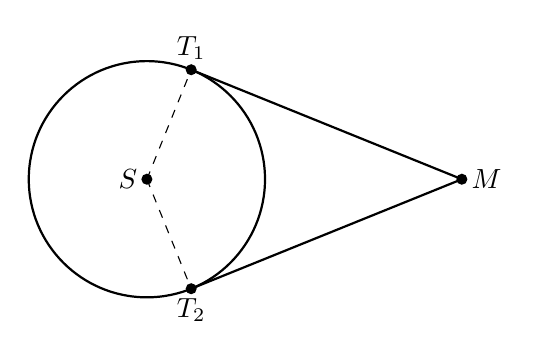
\begin{tikzpicture}[scale=1]
    \coordinate (S) at (0,0);
    \coordinate (M) at (4,0);
    \coordinate (T1) at (0.5625,1.3905);
    \coordinate (T2) at (0.5625,-1.3905);

    \draw[thick] (S) circle (1.5);
    \draw[thick] (M)--(T1) (M)--(T2);
    \draw[dashed] (S)--(T1) (S)--(T2);

    \fill (S) circle (2pt) node[left] {$S$};
    \fill (M) circle (2pt) node[right] {$M$};
    \fill (T1) circle (2pt) node[above] {$T_1$};
    \fill (T2) circle (2pt) node[below] {$T_2$};
\end{tikzpicture}
\end{center}

Rovnost délek plyne například ze shodnosti pravoúhlých trojúhelníků $SMT_1$ a $SMT_2$, které mají společnou přeponu
$SM$ a shodné odvěsny $ST_1=ST_2=r$.

\subsection{Vzájemná poloha dvou kružnic}

Uvažujme dvě kružnice
\[
    k_1(S_1;r_1), \qquad k_2(S_2;r_2)
\]
a označme vzdálenost jejich středů
\[
    d=|S_1S_2|.
\]
Úsečku $S_1S_2$ nazýváme \textbf{středná}. Počet společných bodů obou kružnic lze určit pouze porovnáním vzdálenosti
$d$ s jejich poloměry.

\begin{definitionbox}
    Pro dvě kružnice s různými středy platí:
    \[
    \begin{array}{c|c}
        \text{podmínka} & \text{vzájemná poloha} \\
        \hline
        d>r_1+r_2 & \text{kružnice leží vně sebe, bez společného bodu} \\
        d=r_1+r_2 & \text{vnější dotyk} \\
        |r_1-r_2|<d<r_1+r_2 & \text{dva společné body} \\
        d=|r_1-r_2| & \text{vnitřní dotyk} \\
        0<d<|r_1-r_2| & \text{jedna kružnice leží uvnitř druhé, bez společného bodu}
    \end{array}
    \]
\end{definitionbox}

Jestliže mají kružnice společný střed, tedy $d=0$, nazýváme je \important{soustředné}. Mají-li navíc stejné poloměry,
jsou totožné a mají všechny body společné. Mají-li různé poloměry, nemají žádný společný bod.

\subsection{Mezikruží}

Dvě soustředné kružnice s různými poloměry vymezují oblast, kterou nazýváme \important{mezikruží}. Nechť vnitřní
kružnice má poloměr $r$ a vnější kružnice poloměr $R$, kde $0<r<R$. Potom mezikruží tvoří právě ty body $X$, pro které
platí
\[
    r\leq |SX|\leq R.
\]
Rozdíl poloměrů
\[
    R-r
\]
nazýváme \textbf{šířkou mezikruží}.

\begin{center}
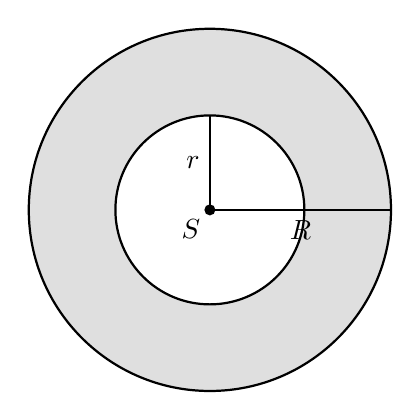
\begin{tikzpicture}[scale=1]
    \fill[gray!25, even odd rule] (0,0) circle (2.3) (0,0) circle (1.2);
    \draw[thick] (0,0) circle (2.3);
    \draw[thick] (0,0) circle (1.2);
    \fill (0,0) circle (2pt) node[below left] {$S$};
    \draw[thick] (0,0)--(2.3,0) node[midway, below] {$R$};
    \draw[thick] (0,0)--(0,1.2) node[midway, left] {$r$};
\end{tikzpicture}
\end{center}

Část mezikruží vymezenou dvěma poloměry a příslušnými oblouky obou kružnic nazýváme \textbf{výseč mezikruží}.

\begin{notebox}
    Kružnice a kruh v této části slouží především k zavedení základních pojmů a vzájemných poloh. Na tyto poznatky
    později navážeme při studiu středových a obvodových úhlů, Thaletovy věty a mocnosti bodu ke kružnici.
\end{notebox}




% -----------------------------------------------------------------
% ---------------------- P Ř Í K L A D Y --------------------------
% -----------------------------------------------------------------

\exercisepart

\setcounter{section}{1}


% =========================
% ÚLOHA 1 – Základní geometrické pojmy
% =========================

\begin{exercise}[Rozhodněte o správnosti následujících tvrzení]

    Rozhodněte, zda jsou následující tvrzení pravdivá. Nepravdivá tvrzení opravte.

    \begin{tasks}(2)
        \task Dvěma různými body prochází právě jedna přímka.
        \task Třemi různými body prochází vždy právě jedna přímka.
        \task Úsečka má dva krajní body.
        \task Polopřímka má právě jeden počáteční bod.
        \task Přímka má dva krajní body.
        \task Dvě různé rovnoběžné přímky nemají žádný společný bod.
        \task Dvě různoběžné přímky mají právě jeden společný bod.
        \task Každé dvě kolmé přímky jsou různoběžné.
        \task Každé dvě různoběžné přímky jsou kolmé.
        \task Přímka rozděluje rovinu na dvě poloroviny.
    \end{tasks}

\end{exercise}


% =========================
% ÚLOHA 2 – Množiny bodů dané vlastnosti
% =========================

\begin{exercise}[Narýsujte množiny bodů dané vlastnosti]

    Je dána úsečka $AB$, pro kterou platí $|AB|=6\,\mathrm{cm}$.
    Narýsujte následující množiny bodů v rovině:

    \begin{tasks}(1)
        \task
        \[
            M_1=\{X;\ |AX|=2\,\mathrm{cm}\}.
        \]

        \task
        \[
            M_2=\{X;\ |AX|\leq 4\,\mathrm{cm}\}.
        \]

        \task
        \[
            M_3=\{X;\ |AX|\leq 4\,\mathrm{cm}
            \land |BX|\leq 4\,\mathrm{cm}\}.
        \]

        \task
        \[
            M_4=\{X;\ |AX|=|BX|\}.
        \]

        \task
        \[
            M_5=\{X;\ |AX|\leq |BX|\}.
        \]

        \task
        \[
            M_6=\{X;\ |AX|=3\,\mathrm{cm}
            \land |BX|=5\,\mathrm{cm}\}.
        \]
    \end{tasks}

\end{exercise}


% =========================
% ÚLOHA 3 – Vzdálenost bodu od přímky
% =========================

\begin{exercise}[Narýsujte množiny bodů se zadanou vzdáleností od přímky]

    Je dána přímka $p$ a kladné reálné číslo $m$.
    Popište a narýsujte množinu všech bodů $X$, pro které platí:

    \begin{tasks}(2)
        \task $d(X,p)=m$
        \task $d(X,p)<m$
        \task $d(X,p)\leq m$
        \task $d(X,p)>m$
    \end{tasks}

\end{exercise}


% =========================
% ÚLOHA 4 – Vzdálenost od dvou přímek
% =========================

\begin{exercise}[Určete množinu bodů stejně vzdálených od dvou přímek]

    Jsou dány dvě různé přímky $p$ a $q$.
    Narýsujte množinu všech bodů $X$, pro které platí
    \[
        d(X,p)=d(X,q),
    \]
    jestliže:

    \begin{tasks}(2)
        \task $p\parallel q$,
        \task $p$ a $q$ jsou různoběžné.
    \end{tasks}

\end{exercise}


% =========================
% ÚLOHA 5 – Vzájemná poloha přímek
% =========================

\begin{exercise}[Určete vzájemnou polohu přímek]

    Rozhodněte, jaký vztah mezi přímkami $p$ a $q$ vyplývá z uvedených podmínek.

    \begin{tasks}(2)
        \task $p\perp r$, $q\perp r$
        \task $p\parallel r$, $q\parallel r$
        \task $p\parallel r$, $q\perp r$
        \task $p\perp q$, $q\perp r$
        \task $p\parallel q$ a $q\neq p$
        \task $p\cap q=\{P\}$
    \end{tasks}

\end{exercise}


% =========================
% ÚLOHA 6 – Vrcholové a vedlejší úhly
% =========================

\begin{exercise}[Dopočítejte velikosti úhlů]

    Přímky $p$ a $q$ jsou různoběžné. Jeden z úhlů, který svírají, má uvedenou velikost.
    Určete velikosti zbývajících tří úhlů.

    \begin{tasks}(2)
        \task $38^\circ$
        \task $72^\circ$
        \task $90^\circ$
        \task $127^\circ$
        \task $151^\circ$
        \task $35^\circ 20'$
    \end{tasks}

\end{exercise}


% =========================
% ÚLOHA 7 – Střídavé, souhlasné a vedlejší úhly
% =========================

\begin{exercise}[Určete velikosti vyznačených úhlů]

    Na obrázku platí $p\parallel q$. Určete velikosti úhlů
    $\alpha$, $\beta$, $\gamma$ a $\delta$.

    \begin{center}
        \begin{tikzpicture}[scale=0.9]
            \draw (-4,1.5) -- (4,1.5) node[right] {$p$};
            \draw (-4,-1.5) -- (4,-1.5) node[right] {$q$};

            \draw (-2.2,-2.5) -- (-0.7,2.5);
            \draw (1.0,-2.5) -- (2.3,2.5);

            \node at (-1.15,1.1) {$68^\circ$};
            \node at (-1.8,-1.1) {$\alpha$};

            \node at (1.25,-1.1) {$\beta$};
            \node at (1.75,1.05) {$\gamma$};
            \node at (2.15,1.95) {$\delta$};
        \end{tikzpicture}
    \end{center}

\end{exercise}


% ================================================================
% 2 – TROJÚHELNÍKY
% ================================================================

\setcounter{section}{2}

% =========================
% ÚLOHA 8 – Druhy trojúhelníků
% =========================

\begin{exercise}[Zařaďte trojúhelníky]

    U každého trojúhelníku určete jeho druh podle délek stran a podle velikostí úhlů,
    pokud je takové určení z uvedených údajů možné.

    \begin{tasks}(2)
        \task $a=5$, $b=5$, $c=6$
        \task $a=b=c=4$
        \task $\alpha=90^\circ$, $\beta=45^\circ$
        \task $\alpha=35^\circ$, $\beta=65^\circ$
        \task $\alpha=120^\circ$, $a=b$
        \task $\alpha=\beta=\gamma$
        \task $a=b$, $\gamma=90^\circ$
        \task $\alpha=40^\circ$, $\beta=40^\circ$
    \end{tasks}

\end{exercise}


% =========================
% ÚLOHA 9 – Trojúhelníková nerovnost
% =========================

\begin{exercise}[Určete možné délky třetí strany]

    V trojúhelníku $ABC$ jsou známy délky dvou stran. Určete všechny možné hodnoty
    délky třetí strany.

    \begin{tasks}(2)
        \task $a=6\,\mathrm{cm}$, $b=8\,\mathrm{cm}$
        \task $a=4\,\mathrm{cm}$, $b=7\,\mathrm{cm}$
        \task $a=12\,\mathrm{cm}$, $b=5\,\mathrm{cm}$
        \task $a=3{,}5\,\mathrm{cm}$, $b=8\,\mathrm{cm}$
        \task $a=10\,\mathrm{cm}$, $b=10\,\mathrm{cm}$
        \task $a=2{,}4\,\mathrm{cm}$, $b=6{,}1\,\mathrm{cm}$
    \end{tasks}

\end{exercise}


% =========================
% ÚLOHA 10 – Existence trojúhelníku
% =========================

\begin{exercise}[Rozhodněte, zda lze trojúhelník sestrojit]

    Rozhodněte, zda existuje trojúhelník s uvedenými délkami stran.

    \begin{tasks}(2)
        \task $3\,\mathrm{cm}$, $4\,\mathrm{cm}$, $5\,\mathrm{cm}$
        \task $2\,\mathrm{cm}$, $3\,\mathrm{cm}$, $6\,\mathrm{cm}$
        \task $5\,\mathrm{cm}$, $5\,\mathrm{cm}$, $10\,\mathrm{cm}$
        \task $6\,\mathrm{cm}$, $7\,\mathrm{cm}$, $12\,\mathrm{cm}$
        \task $1{,}5\,\mathrm{cm}$, $2{,}5\,\mathrm{cm}$, $3\,\mathrm{cm}$
        \task $4\,\mathrm{cm}$, $9\,\mathrm{cm}$, $13\,\mathrm{cm}$
        \task $8\,\mathrm{cm}$, $10\,\mathrm{cm}$, $15\,\mathrm{cm}$
        \task $0{,}8\,\mathrm{cm}$, $1{,}2\,\mathrm{cm}$, $2\,\mathrm{cm}$
    \end{tasks}

\end{exercise}


% =========================
% ÚLOHA 11 – Rovnoramenný trojúhelník
% =========================

\begin{exercise}[Určete možné délky základny]

    Rameno rovnoramenného trojúhelníku má délku $10\,\mathrm{cm}$.
    Určete, jakých hodnot může nabývat délka jeho základny.

\end{exercise}


% =========================
% ÚLOHA 12 – Součet úhlů v trojúhelníku
% =========================

\begin{exercise}[Určete zbývající vnitřní úhly trojúhelníku]

    \begin{tasks}(2)
        \task $\alpha=45^\circ$, $\beta=70^\circ$
        \task $\alpha=90^\circ$, $\beta=32^\circ$
        \task $\alpha=110^\circ$, $\beta=25^\circ$
        \task $\alpha=\beta=55^\circ$
        \task $\alpha=2\beta$, $\gamma=60^\circ$
        \task $\alpha:\beta:\gamma=2:3:4$
        \task $\alpha=\beta$, $\gamma=36^\circ$
        \task $\beta=\alpha+20^\circ$, $\gamma=70^\circ$
    \end{tasks}

\end{exercise}


% =========================
% ÚLOHA 13 – Důkazy s úhly v trojúhelníku
% =========================

\begin{exercise}[Dokažte následující tvrzení]

    \begin{tasks}(1)
        \task Součet velikostí vnitřních úhlů libovolného trojúhelníku je $180^\circ$.

        \task V rovnostranném trojúhelníku mají všechny vnitřní úhly velikost $60^\circ$.

        \task Jestliže jsou v trojúhelníku dva vnitřní úhly shodné, potom jsou shodné také strany ležící proti těmto úhlům.

        \task Průsečík os vnitřních úhlů $\alpha$ a $\beta$ trojúhelníku $ABC$
        označme $O$. Dokažte, že
        \[
            |\angle AOB|=90^\circ+\frac{\gamma}{2}.
        \]
    \end{tasks}

\end{exercise}


% =========================
% ÚLOHA 14 – Výšky, těžnice a střední příčky
% =========================

\begin{exercise}[Určete správná tvrzení]

    Rozhodněte, která tvrzení platí pro každý trojúhelník.

    \begin{tasks}(2)
        \task Tři těžnice se protínají v jednom bodě.
        \task Tři výšky se vždy protínají uvnitř trojúhelníku.
        \task Těžiště leží vždy uvnitř trojúhelníku.
        \task Střední příčka je rovnoběžná s třetí stranou.
        \task Střední příčka má stejnou délku jako třetí strana.
        \task Těžiště dělí těžnici v poměru $2:1$.
        \task V pravoúhlém trojúhelníku leží ortocentrum ve vrcholu pravého úhlu.
        \task V tupoúhlém trojúhelníku leží ortocentrum vně trojúhelníku.
    \end{tasks}

\end{exercise}


% =========================
% ÚLOHA 15 – Střední příčka
% =========================

\begin{exercise}[Vypočítejte délky středních příček]

    \begin{tasks}(2)
        \task $a=8\,\mathrm{cm}$; určete délku střední příčky rovnoběžné se stranou $a$.
        \task $b=13\,\mathrm{cm}$; určete délku střední příčky rovnoběžné se stranou $b$.
        \task Střední příčka má délku $4{,}5\,\mathrm{cm}$; určete délku příslušné strany.
        \task Střední příčka má délku $7\,\mathrm{cm}$; určete délku příslušné strany.
    \end{tasks}

\end{exercise}


% =========================
% ÚLOHA 16 – Těžiště
% =========================

\begin{exercise}[Využijte vlastnosti těžiště]

    Bod $T$ je těžiště trojúhelníku $ABC$ a $S_a$ je střed strany $BC$.

    \begin{tasks}(2)
        \task $|AS_a|=12\,\mathrm{cm}$. Určete $|AT|$ a $|TS_a|$.
        \task $|AT|=8\,\mathrm{cm}$. Určete délku těžnice $t_a$.
        \task $|TS_a|=3{,}5\,\mathrm{cm}$. Určete $|AT|$.
        \task $t_a=15\,\mathrm{cm}$. Určete vzdálenost těžiště od středu strany $BC$.
    \end{tasks}

\end{exercise}


% =========================
% ÚLOHA 17 – Kružnice spojené s trojúhelníkem
% =========================

\begin{exercise}[Doplňte správný geometrický pojem]

    \begin{tasks}(2)
        \task Průsečík os stran trojúhelníku je střed \dots
        \task Průsečík os vnitřních úhlů je střed \dots
        \task Kružnice procházející všemi vrcholy trojúhelníku se nazývá \dots
        \task Kružnice dotýkající se všech tří stran trojúhelníku se nazývá \dots
        \task Trojúhelník má právě \dots kružnice připsané.
        \task Střed kružnice připsané leží v průsečíku os \dots
    \end{tasks}

\end{exercise}


% ================================================================
% 3 – MNOHOÚHELNÍKY
% ================================================================

\setcounter{section}{3}

% =========================
% ÚLOHA 18 – Mnohoúhelníky
% =========================

\begin{exercise}[Určete počet úhlopříček mnohoúhelníku]

    Použijte vztah
    \[
        u=\frac{n(n-3)}{2}.
    \]

    \begin{tasks}(2)
        \task čtyřúhelník
        \task pětiúhelník
        \task šestiúhelník
        \task osmiúhelník
        \task desetiúhelník
        \task dvanáctiúhelník
    \end{tasks}

\end{exercise}


% =========================
% ÚLOHA 19 – Obrácená úloha s úhlopříčkami
% =========================

\begin{exercise}[Určete počet stran mnohoúhelníku]

    Určete počet stran mnohoúhelníku, jestliže má:

    \begin{tasks}(2)
        \task $5$ úhlopříček,
        \task $9$ úhlopříček,
        \task $14$ úhlopříček,
        \task $20$ úhlopříček,
        \task $35$ úhlopříček,
        \task $54$ úhlopříček.
    \end{tasks}

\end{exercise}


% =========================
% ÚLOHA 20 – Součet vnitřních úhlů mnohoúhelníku
% =========================

\begin{exercise}[Určete součet velikostí vnitřních úhlů]

    \begin{tasks}(2)
        \task čtyřúhelníku,
        \task pětiúhelníku,
        \task šestiúhelníku,
        \task osmiúhelníku,
        \task desetiúhelníku,
        \task patnáctiúhelníku.
    \end{tasks}

\end{exercise}


% =========================
% ÚLOHA 21 – Pravidelné mnohoúhelníky
% =========================

\begin{exercise}[Určete velikost jednoho vnitřního úhlu pravidelného mnohoúhelníku]

    \begin{tasks}(2)
        \task pravidelný trojúhelník,
        \task čtverec,
        \task pravidelný pětiúhelník,
        \task pravidelný šestiúhelník,
        \task pravidelný osmiúhelník,
        \task pravidelný dvanáctiúhelník.
    \end{tasks}

\end{exercise}


% ================================================================
% 4 – ČTYŘÚHELNÍKY
% ================================================================

\setcounter{section}{4}

% =========================
% ÚLOHA 22 – Čtyřúhelníky
% =========================

\begin{exercise}[Určete všechny možné názvy čtyřúhelníku]

    Pro každý popis určete všechny typy čtyřúhelníků, kterým může daný útvar být.

    \begin{tasks}(1)
        \task Má dvě dvojice rovnoběžných protějších stran.
        \task Má všechny strany stejně dlouhé.
        \task Má všechny vnitřní úhly pravé.
        \task Má všechny strany stejně dlouhé a všechny vnitřní úhly pravé.
        \task Má právě dvě dvojice shodných sousedních stran.
        \task Má alespoň jednu dvojici rovnoběžných protějších stran.
        \task Je rovnoběžníkem a jeho úhlopříčky jsou shodné.
        \task Je rovnoběžníkem a jeho úhlopříčky jsou na sebe kolmé.
    \end{tasks}

\end{exercise}


% =========================
% ÚLOHA 23 – Vlastnosti čtyřúhelníků
% =========================

\begin{exercise}[Rozhodněte, zda tvrzení platí vždy]

    \begin{tasks}(2)
        \task Každý čtverec je obdélník.
        \task Každý obdélník je čtverec.
        \task Každý čtverec je kosočtverec.
        \task Každý kosočtverec je čtverec.
        \task Každý rovnoběžník je lichoběžník.
        \task Každý lichoběžník je rovnoběžník.
        \task Úhlopříčky každého rovnoběžníku se navzájem půlí.
        \task Úhlopříčky každého obdélníku jsou stejně dlouhé.
        \task Úhlopříčky každého kosočtverce jsou kolmé.
        \task Každý čtverec je zároveň deltoid.
    \end{tasks}

\end{exercise}


% =========================
% ÚLOHA 24 – Lichoběžník
% =========================

\begin{exercise}[Vypočítejte délku střední příčky lichoběžníku]

    \begin{tasks}(2)
        \task $a=8\,\mathrm{cm}$, $c=4\,\mathrm{cm}$
        \task $a=12\,\mathrm{cm}$, $c=7\,\mathrm{cm}$
        \task $a=5{,}5\,\mathrm{cm}$, $c=9{,}5\,\mathrm{cm}$
        \task $a=14\,\mathrm{cm}$, $c=6\,\mathrm{cm}$
    \end{tasks}

\end{exercise}


% ================================================================
% 5 – KRUŽNICE A KRUH
% ================================================================

\setcounter{section}{5}

% =========================
% ÚLOHA 25 – Základní pojmy kružnice
% =========================

\begin{exercise}[Doplňte správný pojem]

    \begin{tasks}(2)
        \task Úsečka spojující dva body kružnice se nazývá \dots
        \task Tětiva procházející středem kružnice se nazývá \dots
        \task Část kružnice mezi dvěma body se nazývá \dots
        \task Část kruhu ohraničená dvěma poloměry a obloukem se nazývá \dots
        \task Část kruhu ohraničená tětivou a obloukem se nazývá \dots
        \task Průměr kružnice o poloměru $r$ má délku \dots
    \end{tasks}

\end{exercise}


% =========================
% ÚLOHA 26 – Kružnice a kruh
% =========================

\begin{exercise}[Rozhodněte, kde leží bod $X$]

    Je dána kružnice $k(S;5\,\mathrm{cm})$ a kruh $K(S;5\,\mathrm{cm})$.
    Rozhodněte, zda bod $X$ leží uvnitř kruhu, na kružnici, nebo vně kruhu, jestliže:

    \begin{tasks}(2)
        \task $|SX|=3\,\mathrm{cm}$
        \task $|SX|=5\,\mathrm{cm}$
        \task $|SX|=7\,\mathrm{cm}$
        \task $|SX|=4{,}99\,\mathrm{cm}$
        \task $|SX|=5{,}01\,\mathrm{cm}$
        \task $X=S$
    \end{tasks}

\end{exercise}


% =========================
% ÚLOHA 27 – Přímka a kružnice
% =========================

\begin{exercise}[Určete vzájemnou polohu přímky a kružnice]

    Je dána kružnice $k(S;r)$ a přímka $p$. Rozhodněte, zda je přímka $p$
    sečnou, tečnou nebo vnější přímkou kružnice.

    \begin{tasks}(2)
        \task $r=5\,\mathrm{cm}$, $d(S,p)=3\,\mathrm{cm}$
        \task $r=4\,\mathrm{cm}$, $d(S,p)=4\,\mathrm{cm}$
        \task $r=6\,\mathrm{cm}$, $d(S,p)=8\,\mathrm{cm}$
        \task $r=2{,}5\,\mathrm{cm}$, $d(S,p)=2\,\mathrm{cm}$
        \task $r=7\,\mathrm{cm}$, $d(S,p)=7\,\mathrm{cm}$
        \task $r=3\,\mathrm{cm}$, $d(S,p)=3{,}1\,\mathrm{cm}$
    \end{tasks}

\end{exercise}


% =========================
% ÚLOHA 28 – Tětiva
% =========================

\begin{exercise}[Využijte vlastnost kolmice na tětivu]

    Na kružnici $k(S;r)$ leží body $A$ a $B$. Bod $P$ je pata kolmice
    vedené ze středu $S$ na tětivu $AB$.

    \begin{tasks}(2)
        \task $|AB|=10\,\mathrm{cm}$. Určete $|AP|$.
        \task $|AP|=3{,}5\,\mathrm{cm}$. Určete $|AB|$.
        \task $|PB|=6\,\mathrm{cm}$. Určete $|AP|$.
        \task $|AB|=15\,\mathrm{cm}$. Určete $|PB|$.
    \end{tasks}

\end{exercise}


% =========================
% ÚLOHA 29 – Tečna ke kružnici
% =========================

\begin{exercise}[Rozhodněte, zda je přímka tečnou]

    Je dána kružnice $k(S;r)$, bod $T$ na kružnici a přímka $p$ procházející bodem $T$.
    Rozhodněte, zda je $p$ tečnou kružnice.

    \begin{tasks}(2)
        \task $ST\perp p$
        \task $|\angle STp|=70^\circ$
        \task $|\angle STp|=90^\circ$
        \task $|\angle STp|=45^\circ$
    \end{tasks}

\end{exercise}


% =========================
% ÚLOHA 30 – Tečny z vnějšího bodu
% =========================

\begin{exercise}[Využijte vlastnosti tečen vedených z jednoho bodu]

    Z bodu $M$ ležícího vně kružnice jsou vedeny tečny s body dotyku $T_1$ a $T_2$.

    \begin{tasks}(2)
        \task $|MT_1|=7\,\mathrm{cm}$. Určete $|MT_2|$.
        \task $|MT_2|=4{,}5\,\mathrm{cm}$. Určete $|MT_1|$.
        \task $|MT_1|+|MT_2|=18\,\mathrm{cm}$. Určete délku každé tečnové úsečky.
        \task $|MT_1|-|MT_2|=0$. Vysvětlete, proč tato rovnost platí vždy.
    \end{tasks}

\end{exercise}


% =========================
% ÚLOHA 31 – Vzájemná poloha dvou kružnic
% =========================

\begin{exercise}[Určete vzájemnou polohu dvou kružnic]

    Pro každou dvojici kružnic určete počet společných bodů a jejich vzájemnou polohu.

    \begin{tasks}(1)
        \task $r_1=5\,\mathrm{cm}$, $r_2=2\,\mathrm{cm}$, $|S_1S_2|=9\,\mathrm{cm}$.
        \task $r_1=5\,\mathrm{cm}$, $r_2=2\,\mathrm{cm}$, $|S_1S_2|=7\,\mathrm{cm}$.
        \task $r_1=5\,\mathrm{cm}$, $r_2=2\,\mathrm{cm}$, $|S_1S_2|=6\,\mathrm{cm}$.
        \task $r_1=5\,\mathrm{cm}$, $r_2=2\,\mathrm{cm}$, $|S_1S_2|=3\,\mathrm{cm}$.
        \task $r_1=5\,\mathrm{cm}$, $r_2=2\,\mathrm{cm}$, $|S_1S_2|=1\,\mathrm{cm}$.
        \task $r_1=5\,\mathrm{cm}$, $r_2=5\,\mathrm{cm}$, $|S_1S_2|=0$.
    \end{tasks}

\end{exercise}


% =========================
% ÚLOHA 32 – Určete možnou vzdálenost středů
% =========================

\begin{exercise}[Určete podmínku pro vzdálenost středů kružnic]

    Kružnice mají poloměry
    \[
        r_1=7\,\mathrm{cm},
        \qquad
        r_2=3\,\mathrm{cm}.
    \]
    Určete, jakou podmínku musí splňovat vzdálenost $d=|S_1S_2|$, aby:

    \begin{tasks}(1)
        \task kružnice neměly žádný společný bod a ležely vně sebe,
        \task měly vnější dotyk,
        \task měly dva společné body,
        \task měly vnitřní dotyk,
        \task jedna kružnice ležela uvnitř druhé a neměly společný bod.
    \end{tasks}

\end{exercise}


% =========================
% ÚLOHA 33 – Mezikruží
% =========================

\begin{exercise}[Pracujte s mezikružím]

    Jsou dány dvě soustředné kružnice se společným středem $S$ a poloměry
    $r=3\,\mathrm{cm}$ a $R=8\,\mathrm{cm}$.

    \begin{tasks}(2)
        \task Určete šířku mezikruží.
        \task Rozhodněte, zda bod $X$, pro který $|SX|=6\,\mathrm{cm}$, leží v mezikruží.
        \task Rozhodněte, zda bod $Y$, pro který $|SY|=2\,\mathrm{cm}$, leží v mezikruží.
        \task Rozhodněte, zda bod $Z$, pro který $|SZ|=8\,\mathrm{cm}$, leží v mezikruží.
    \end{tasks}

\end{exercise}


% ================================================================
% 6 – KONSTRUKČNÍ ÚLOHY
% ================================================================

\setcounter{section}{6}

% =========================
% ÚLOHA 34 – Konstrukce tečen ke kružnici
% =========================

\begin{exercise}[Sestrojte tečny z bodu ke kružnici]

    Je dána kružnice $k(S;3\,\mathrm{cm})$ a bod $M$, pro který
    \[
        |SM|=7\,\mathrm{cm}.
    \]
    Sestrojte obě tečny vedené bodem $M$ ke kružnici $k$ a vyznačte jejich body dotyku.

\end{exercise}


% =========================
% ÚLOHA 35 – Konstrukce kružnic daného poloměru
% =========================

\begin{exercise}[Sestrojte kružnice požadovaných vlastností]

    Je dána kružnice $k(O;4\,\mathrm{cm})$ a bod $M$.
    Sestrojte všechny kružnice o poloměru $1{,}5\,\mathrm{cm}$,
    které se dotýkají kružnice $k$ a procházejí bodem $M$, jestliže:

    \begin{tasks}(2)
        \task $|OM|=3\,\mathrm{cm}$,
        \task $|OM|=1\,\mathrm{cm}$,
        \task $|OM|=0{,}5\,\mathrm{cm}$,
        \task $|OM|=5\,\mathrm{cm}$.
    \end{tasks}

\end{exercise}


% =========================
% ÚLOHA 36 – Konstrukce kružnice dotýkající se přímky
% =========================

\begin{exercise}[Sestrojte kružnice dotýkající se kružnice a přímky]

    Je dána kružnice $k(O;4\,\mathrm{cm})$ a přímka $p$.
    Sestrojte všechny kružnice o poloměru $1{,}5\,\mathrm{cm}$,
    které se dotýkají kružnice $k$ i přímky $p$, jestliže:

    \begin{tasks}(2)
        \task $d(O,p)=3\,\mathrm{cm}$,
        \task $d(O,p)=0{,}5\,\mathrm{cm}$.
    \end{tasks}

\end{exercise}


% =========================
% ÚLOHA 37 – Konstrukce kružnic mezi rovnoběžkami
% =========================

\begin{exercise}[Sestrojte kružnice dotýkající se dvou rovnoběžek]

    Jsou dány dvě rovnoběžné přímky $p_1$, $p_2$, jejichž vzdálenost je
    $4\,\mathrm{cm}$, a bod $M$, pro který
    \[
        d(M,p_1)=1\,\mathrm{cm}.
    \]
    Sestrojte všechny kružnice, které se dotýkají obou přímek
    $p_1$, $p_2$ a procházejí bodem $M$.

\end{exercise}


% =========================
% ÚLOHA 38 – Konstrukce trojúhelníků
% =========================

\begin{exercise}[Sestrojte trojúhelníky podle zadaných prvků]

    Ve všech úlohách sestrojte všechny trojúhelníky $ABC$, které splňují uvedené podmínky.

    \begin{tasks}(1)
        \task $c=6\,\mathrm{cm}$, $v_c=2\,\mathrm{cm}$, $t_c=4\,\mathrm{cm}$.
        \task $c=6\,\mathrm{cm}$, $v_c=3\,\mathrm{cm}$, $t_c=4\,\mathrm{cm}$.
        \task $c=5\,\mathrm{cm}$, $\alpha=60^\circ$, $t_c=5{,}5\,\mathrm{cm}$.
        \task $c=5\,\mathrm{cm}$, $\beta=120^\circ$, $v_c=5\,\mathrm{cm}$.
    \end{tasks}

\end{exercise}


% =========================
% ÚLOHA 39 – Souhrnné konstrukce trojúhelníků
% =========================

\begin{exercise}[Souhrnné konstrukce trojúhelníků]

    V trojúhelníku $ABC$ označujeme délky stran $a$, $b$, $c$, velikosti vnitřních úhlů
    $\alpha$, $\beta$, $\gamma$, výšky $v_a$, $v_b$, $v_c$, ortocentrum $V$,
    těžnice $t_a$, $t_b$, $t_c$, těžiště $T$, poloměr kružnice opsané $r$
    a poloměr kružnice vepsané $\rho$.

    U každé následující konstrukce proveďte \textbf{náčrt, rozbor, konstrukci, popis postupu konstrukce
    a diskusi počtu řešení}. Uvažujte všechny přípustné volby zadaných veličin.

    Sestrojte všechny trojúhelníky $ABC$, jsou-li dány následující prvky; úlohy jsou seřazeny
    přibližně od jednodušších k náročnějším:

    \begin{tasks}(1)
        \task $a,\,b,\,c$
        \task $\alpha,\,\beta,\,\gamma$
        \task $\alpha,\,b,\,c$
        \task $a,\,b,\,v_c$
        \task $a,\,b,\,v_a$
        \task $a,\,b,\,t_a$
        \task $a,\,v_a,\,t_a$
        \task $c,\,v_a,\,t_a$
        \task $a,\,v_a,\,v_b$
        \task $a,\,b,\,r$
        \task $\beta,\,v_a,\,\rho$
        \task $a,\,v_a,\,t_a$
        \task $t_a,\,t_b,\,t_c$
        \task $\alpha,\,v_a,\,c$
        \task $\alpha,\,a,\,v_c$
        \task $\alpha,\,v_b,\,t_a$
        \task $\gamma,\,v_c,\,c$
        \task $\alpha,\,v_a,\,t_a$
        \task $\gamma,\,v_a,\,v_c$
        \task $c,\,\gamma,\,r$
        \task $\rho,\,\alpha,\,v_b$
        \task $\rho,\,\alpha,\,\beta$
        \task $c,\,v_a,\,r$
        \task $v_a,\,\gamma,\,r$
        \task $a,\,\alpha,\,\rho$
        \task $t_c,\,v_c,\,u_c$, kde $u_c$ označuje délku osy úhlu $\gamma$ od vrcholu $C$
        k jejímu průsečíku se stranou $AB$.
    \end{tasks}

\end{exercise}


% ================================================================
% 7 – APLIKAČNÍ A ROZŠIŘUJÍCÍ ÚLOHY
% ================================================================

\setcounter{section}{7}

% =========================
% ÚLOHA 40 – Smíšené úlohy
% =========================

\begin{exercise}[Vyřešte následující úlohy]

    \begin{tasks}(1)
        \task
        V rovnostranném trojúhelníku $ABC$ zvolte body
        $K\in AB$, $L\in BC$, $M\in CA$ tak, aby platilo
        \[
            |AK|=|BL|=|CM|.
        \]
        Dokažte, že trojúhelník $KLM$ je rovnostranný.

        \task
        Na kružnici jsou dány body $A$ a $B$. Vyznačte tětivu $AB$,
        menší a větší oblouk $AB$, obě kruhové úseče a obě kruhové výseče
        určené body $A$, $B$ a středem kružnice.

        \task
        Jsou dány kružnice $k_1(S_1;4\,\mathrm{cm})$ a
        $k_2(S_2;2\,\mathrm{cm})$. Určete všechny hodnoty vzdálenosti
        $|S_1S_2|$, pro které mají kružnice právě jeden společný bod.

        \task
        Průměr kružnice má délku $14\,\mathrm{cm}$.
        Určete její poloměr a rozhodněte, jakou vzájemnou polohu má s kružnicí
        o poloměru $5\,\mathrm{cm}$, jestliže vzdálenost jejich středů je
        $12\,\mathrm{cm}$.
    \end{tasks}

\end{exercise}


% =========================
% ÚLOHA 41 – Obsah obrazce složeného ze čtverce a kruhu
% =========================

\begin{exercise}[Určete obsahy částí obrazce]

    Obrazec je tvořen čtvercem a kruhem, které se částečně překrývají.
    Obsah jejich společné části je $12\,\mathrm{cm}^2$. Tato společná část tvoří
    dvě třetiny obsahu čtverce a současně jednu čtvrtinu obsahu kruhu.

    \begin{center}
        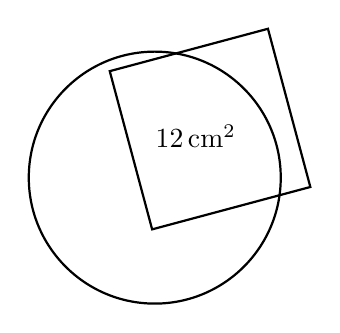
\begin{tikzpicture}[scale=0.8]
            \draw[thick] (0,0) circle (2);

            \begin{scope}[rotate around={15:(1,0.7)}]
                \draw[thick] (-0.4,-0.5) rectangle (2.2,2.1);
            \end{scope}

            \node at (0.65,0.65) {$12\,\mathrm{cm}^2$};
        \end{tikzpicture}
    \end{center}

    \begin{tasks}(1)
        \task Vypočítejte obsah celého obrazce, tedy obsah sjednocení čtverce a kruhu.
        \task Vyjádřete poměr obsahu čtverce a obsahu kruhu v tomto pořadí.
    \end{tasks}

\end{exercise}


% =========================
% ÚLOHA 42 – Rozdělení čtverce na tři části
% =========================

\begin{exercise}[Rozhodněte o pravdivosti tvrzení]

    Čtverec o straně délky $4{,}5\,\mathrm{cm}$ je rozdělen na tři části
    označené $A$, $B$ a $C$. Bod na horní straně je vzdálen
    $3\,\mathrm{cm}$ od levého horního vrcholu a bod na levé straně je
    vzdálen $3\,\mathrm{cm}$ od levého dolního vrcholu.

    \begin{center}
        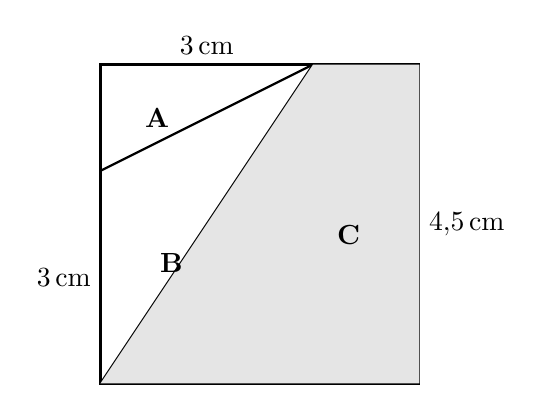
\begin{tikzpicture}[scale=0.9]
            \coordinate (L) at (0,0);
            \coordinate (R) at (4.5,0);
            \coordinate (T) at (4.5,4.5);
            \coordinate (U) at (0,4.5);
            \coordinate (P) at (3,4.5);
            \coordinate (Q) at (0,3);

            \draw[thick] (L)--(R)--(T)--(U)--cycle;
            \draw[thick] (Q)--(P);
            \draw[thick] (L)--(P);

            \fill[gray!20] (P)--(T)--(R)--(L)--cycle;

            \node at (0.8,3.75) {\textbf{A}};
            \node at (1.0,1.7) {\textbf{B}};
            \node at (3.5,2.1) {\textbf{C}};

            \node[above] at (1.5,4.5) {$3\,\mathrm{cm}$};
            \node[left] at (0,1.5) {$3\,\mathrm{cm}$};
            \node[right] at (4.5,2.25) {$4{,}5\,\mathrm{cm}$};
        \end{tikzpicture}
    \end{center}

    Rozhodněte o každém tvrzení, zda je pravdivé.

    \begin{tasks}(1)
        \task Obsahy trojúhelníků $A$ a $B$ jsou v poměru $1:2$.
        \task Obsah trojúhelníku $B$ tvoří dvě devítiny obsahu celého čtverce.
        \task Obsahy obrazců $B$ a $C$ jsou v poměru $1:3$.
    \end{tasks}

\end{exercise}


% =========================
% ÚLOHA 43 – Obsah trojúhelníku a lichoběžníku
% =========================

\begin{exercise}[Určete délku základny lichoběžníku]

    Je dán lichoběžník $ABCD$, kde $AB\parallel CD$, přičemž
    \[
        |AB|=15\,\mathrm{cm}.
    \]
    Bod $Y$ leží uvnitř úsečky $CD$ a obsah trojúhelníku $ABY$
    je roven $\frac56$ obsahu celého lichoběžníku $ABCD$.

    \begin{center}
        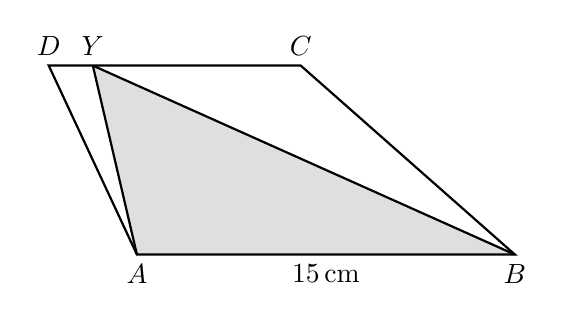
\begin{tikzpicture}[scale=0.8]
            \coordinate (A) at (0,0);
            \coordinate (B) at (6,0);
            \coordinate (D) at (-1.4,3);
            \coordinate (C) at (2.6,3);
            \coordinate (Y) at (-0.7,3);

            \fill[gray!25] (A)--(B)--(Y)--cycle;

            \draw[thick] (A)--(B)--(C)--(D)--cycle;
            \draw[thick] (Y)--(A);
            \draw[thick] (Y)--(B);

            \node[below] at (A) {$A$};
            \node[below] at (B) {$B$};
            \node[above] at (C) {$C$};
            \node[above] at (D) {$D$};
            \node[above] at (Y) {$Y$};

            \node[below] at (3,0) {$15\,\mathrm{cm}$};
        \end{tikzpicture}
    \end{center}

    Vypočítejte délku strany $CD$.

\end{exercise}


% =========================
% ÚLOHA 44 – BONUS
% =========================

\begin{exercise}[BONUS: Určete výšku zdi pomocí stínu]

    Svislá zeď vrhá na vodorovnou podložku stín do vzdálenosti
    $6\,\mathrm{m}$ od zdi. Na podložce stojí bedna tvaru krychle
    o hraně délky $1\,\mathrm{m}$.

    Bednu lze od zdi posunout nejvýše tak, že její bližší stěna je
    ve vzdálenosti
    \[
        d=3{,}75\,\mathrm{m}
    \]
    od zdi, přičemž bedna ještě zůstává celá ve stínu.

    \begin{center}
        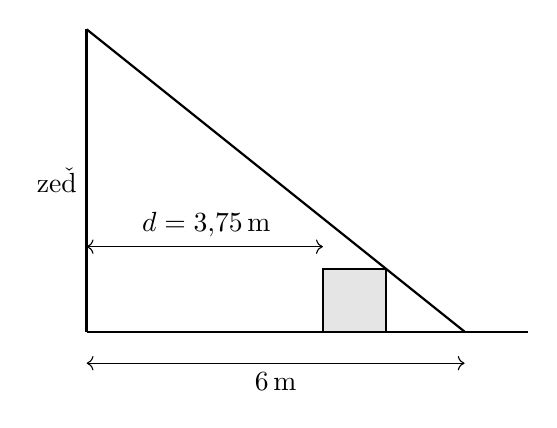
\begin{tikzpicture}[scale=0.8]
            % zem
            \draw[thick] (0,0)--(7,0);

            % zeď
            \draw[very thick] (0,0)--(0,4.8);

            % hranice stínu
            \draw[thick] (0,4.8)--(6,0);

            % bedna
            \filldraw[fill=gray!20, thick]
                (3.75,0) rectangle (4.75,1);

            % délka stínu
            \draw[<->] (0,-0.5)--(6,-0.5);
            \node[below] at (3,-0.5) {$6\,\mathrm{m}$};

            % vzdálenost bedny
            \draw[<->] (0,1.35)--(3.75,1.35);
            \node[above] at (1.9,1.35) {$d=3{,}75\,\mathrm{m}$};

            \node[left] at (0,2.4) {zeď};
        \end{tikzpicture}
    \end{center}

    Jak vysoká je zeď?

\end{exercise}


% =========================
% ÚLOHA 45 – BONUS
% =========================

\begin{exercise}[BONUS: Určete obsah trojúhelníku pomocí podobnosti]

    Platí
    \[
        AB\parallel DE,
        \qquad
        |AB|=6\,\mathrm{cm},
        \qquad
        |DE|=4\,\mathrm{cm}.
    \]
    Přímky $AD$ a $BE$ se protínají v bodě $C$ a obsah trojúhelníku
    $CDE$ je
    \[
        S_{\triangle CDE}=4\,\mathrm{cm}^2.
    \]

    \begin{center}
        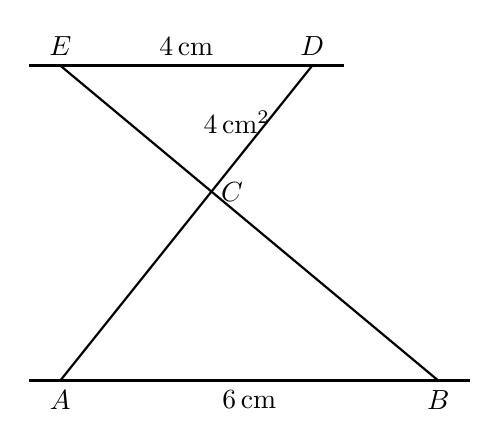
\begin{tikzpicture}[scale=0.8]
            \coordinate (A) at (0,0);
            \coordinate (B) at (6,0);
            \coordinate (C) at (2.4,3);
            \coordinate (D) at (4,5);
            \coordinate (E) at (0,5);

            \draw[thick] (-0.5,0)--(6.5,0);
            \draw[thick] (-0.5,5)--(4.5,5);

            \draw[thick] (A)--(D);
            \draw[thick] (B)--(E);

            \node[below] at (A) {$A$};
            \node[below] at (B) {$B$};
            \node[right] at (C) {$C$};
            \node[above] at (D) {$D$};
            \node[above] at (E) {$E$};

            \node[below] at (3,0) {$6\,\mathrm{cm}$};
            \node[above] at (2,5) {$4\,\mathrm{cm}$};
            \node at (2.8,4.1) {$4\,\mathrm{cm}^2$};
        \end{tikzpicture}
    \end{center}

    Vypočítejte obsah trojúhelníku $ABC$.

\end{exercise}


% =========================
% ÚLOHA 46 – BONUS
% =========================

\begin{exercise}[BONUS: Porovnejte plochy obou částí střechy]

    Dvě části střechy domu mají tvar obdélníků se společnou délkou podél hřebene.
    V příčném řezu svírají obě části střechy úhel $105^\circ$, zatímco levá část
    střechy svírá s vodorovnou rovinou úhel $30^\circ$.

    \begin{center}
        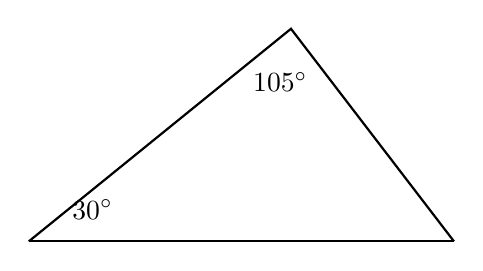
\begin{tikzpicture}[scale=0.9]
            \coordinate (A) at (-3,0);
            \coordinate (B) at (3,0);
            \coordinate (C) at (0.7,3);

            \draw[thick] (A)--(C)--(B);
            \draw[thick] (A)--(B);

            \node at (-2.1,0.45) {$30^\circ$};
            \node at (0.55,2.25) {$105^\circ$};
        \end{tikzpicture}
    \end{center}

    Určete poměr ploch levé a pravé části střechy v tomto pořadí.

\end{exercise}


% =========================
% ÚLOHA 47 – BONUS
% =========================

\begin{exercise}[BONUS: Určete obsah kruhové výseče]

    Z kruhu o poloměru
    \[
        r=6\,\mathrm{cm}
    \]
    je oddělena kruhová výseč. Obvod této výseče je roven
    \[
        o=5r.
    \]

    \begin{center}
        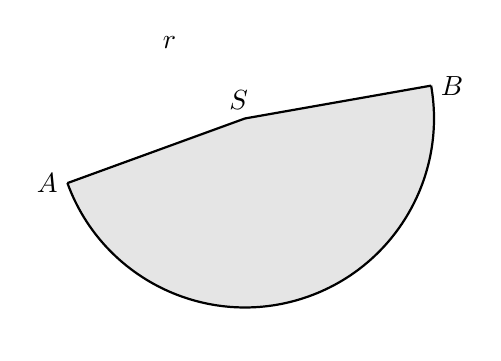
\begin{tikzpicture}[scale=0.8]
            \coordinate (S) at (0,0);
            \coordinate (A) at (200:3);
            \coordinate (B) at (10:3);

            \fill[gray!20] (S)--(A) arc (200:370:3)--cycle;
            \draw[thick] (S)--(A);
            \draw[thick] (S)--(B);
            \draw[thick] (A) arc (200:370:3);

            \node at (-0.1,0.3) {$S$};
            \node[left] at (A) {$A$};
            \node[right] at (B) {$B$};
            \node at (-1.2,1.2) {$r$};
        \end{tikzpicture}
    \end{center}

    Vypočítejte obsah kruhové výseče.

\end{exercise}


% =========================
% ÚLOHA 48 – BONUS
% =========================

\begin{exercise}[BONUS: Elipsa určená ohnisky]

    Na polopřímce $EF$ leží v uvedeném pořadí body
    $A$, $B$, $C$, $D$, $X$ a $Y$. Mimo tuto polopřímku leží bod $M$.
    Uvažujte elipsu s ohnisky $E$, $F$, která prochází bodem $M$.

    Obrázek je určen ke konstrukčnímu řešení.

    \begin{center}
        \begin{tikzpicture}[scale=0.72]
            \coordinate (E) at (0,0);
            \coordinate (F) at (5,0);
            \coordinate (A) at (6,0);
            \coordinate (B) at (7,0);
            \coordinate (C) at (8,0);
            \coordinate (D) at (9,0);
            \coordinate (X) at (10,0);
            \coordinate (Y) at (11,0);
            \coordinate (M) at (4.7,3);

            \draw[thick,->] (E)--(12,0);

            \foreach \P/\name in {
                E/E,F/F,A/A,B/B,C/C,D/D,X/X,Y/Y
            }{
                \draw (\P) ++(0,-0.18)--++(0,0.36);
                \node[below=5pt] at (\P) {$\name$};
            }

            \node at (M) {$\times$};
            \node[right] at (M) {$M$};
        \end{tikzpicture}
    \end{center}

    Určete, na které z úseček
    \[
        AB,\quad BC,\quad CD,\quad DX
    \]
    nebo na polopřímce $XY$ leží druhý průsečík elipsy s polopřímkou $EY$.

\end{exercise}


% =========================
% ÚLOHA 49 – BONUS
% =========================

\begin{exercise}[BONUS: Obsah osově souměrného obrazce v kružnici]

    Do kružnice se středem $S$ a poloměrem $10\,\mathrm{cm}$ je vepsán
    osově souměrný čtyřúhelník znázorněný na obrázku. Bod $V$ leží na kružnici
    a pro vyznačený úhel $\alpha$ platí
    \[
        \cos\alpha=0{,}6.
    \]

    \begin{center}
        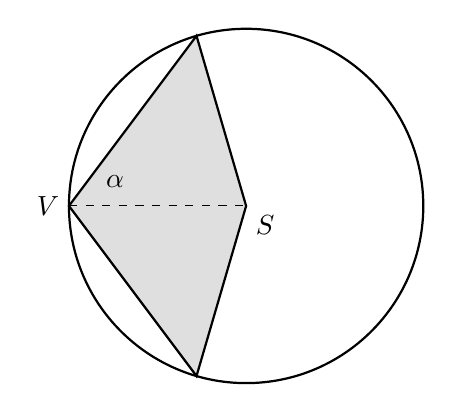
\begin{tikzpicture}[scale=0.9]
            \coordinate (S) at (0,0);
            \coordinate (V) at (-2.5,0);
            \coordinate (T) at (-0.7,2.4);
            \coordinate (B) at (-0.7,-2.4);

            \draw[thick] (S) circle (2.5);

            \filldraw[fill=gray!25, thick]
                (V)--(T)--(S)--(B)--cycle;

            \draw[dashed] (V)--(S);

            \node[left] at (V) {$V$};
            \node[below right] at (S) {$S$};
            \node at (-1.85,0.35) {$\alpha$};
        \end{tikzpicture}
    \end{center}

    Vypočítejte obsah šedého obrazce.

\end{exercise}


% =========================
% ÚLOHA 50 – BONUS
% =========================

\begin{exercise}[BONUS: Obvod pětiúhelníku složeného z kosočtverců]

    Pětiúhelník $ABCDE$ se skládá ze tří shodných kosočtverců
    o straně délky $3\,\mathrm{cm}$ a jednoho tupoúhlého trojúhelníku.
    Pro vyznačený úhel $\alpha$ platí
    \[
        \cos\alpha=\frac19.
    \]

    \begin{center}
        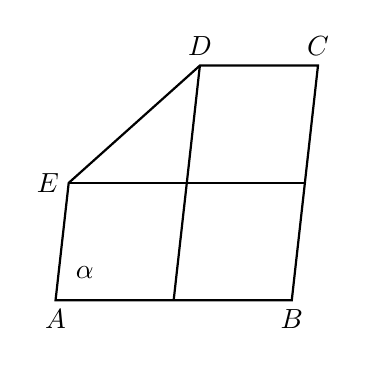
\begin{tikzpicture}[scale=1]
            \coordinate (A) at (0,0);
            \coordinate (P) at (1.5,0);
            \coordinate (B) at (3,0);

            \coordinate (E) at (0.167,1.491);
            \coordinate (Q) at (1.667,1.491);
            \coordinate (R) at (3.167,1.491);

            \coordinate (D) at (1.833,2.981);
            \coordinate (C) at (3.333,2.981);

            \draw[thick] (A)--(B)--(C)--(D)--(E)--cycle;

            \draw[thick] (P)--(Q)--(D);
            \draw[thick] (E)--(Q)--(R);

            \node[below] at (A) {$A$};
            \node[below] at (B) {$B$};
            \node[above] at (C) {$C$};
            \node[above] at (D) {$D$};
            \node[left] at (E) {$E$};

            \node at (0.37,0.35) {$\alpha$};
        \end{tikzpicture}
    \end{center}

    Vypočítejte obvod pětiúhelníku $ABCDE$.

\end{exercise}


% =========================
% ÚLOHA 51 – BONUS
% =========================

\begin{exercise}[BONUS: Poměr obsahů v šestiúhelníku]

    Šestiúhelník $ABCDEF$ je rozdělen na dva bílé rovnoramenné trojúhelníky
    a dva shodné čtverce. Všechny čtyři útvary mají společný vrchol $V$.
    Součet obsahů obou bílých trojúhelníků označme $S_B$ a součet obsahů
    obou čtverců označme $S_T$.

    Úhel $DVE$ má velikost
    \[
        \varphi\in\left(0;\frac{\pi}{2}\right).
    \]

    \begin{center}
        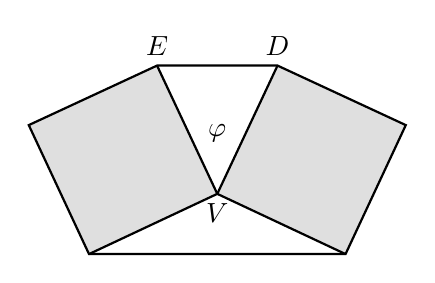
\begin{tikzpicture}[scale=0.9]
            \coordinate (V) at (0,0);
            \coordinate (E) at (-0.85,1.81);
            \coordinate (D) at (0.85,1.81);
            \coordinate (A) at (-1.81,-0.85);
            \coordinate (B) at (1.81,-0.85);
            \coordinate (F) at (-2.66,0.97);
            \coordinate (C) at (2.66,0.97);

            \fill[gray!25] (V)--(E)--(F)--(A)--cycle;
            \fill[gray!25] (V)--(D)--(C)--(B)--cycle;

            \draw[thick]
                (A)--(B)--(C)--(D)--(E)--(F)--cycle;

            \draw[thick] (V)--(A);
            \draw[thick] (V)--(B);
            \draw[thick] (V)--(E);
            \draw[thick] (V)--(D);

            \node[below] at (V) {$V$};
            \node[above] at (E) {$E$};
            \node[above] at (D) {$D$};
            \node at (0,0.85) {$\varphi$};
        \end{tikzpicture}
    \end{center}

    \begin{tasks}(1)
        \task Vyjádřete poměr $S_B:S_T$ v závislosti na velikosti úhlu $\varphi$.
        \task Vypočítejte velikost úhlu $\varphi$, jestliže platí
        \[
            S_B:S_T=1:4.
        \]
    \end{tasks}

\end{exercise}


% =========================
% ÚLOHA 52 – BONUS
% =========================

\begin{exercise}[BONUS: Dvě cesty v obdélníkovém pozemku]

    Obdélníkový pozemek $ABCD$ má rozměry
    \[
        |AB|=360\,\mathrm{m},
        \qquad
        |AD|=480\,\mathrm{m}.
    \]
    Body $M$ a $X$ leží na úhlopříčce $AC$, body $N$ a $Y$ leží
    na stranách obdélníku a úsečky $MN$, $XY$ jsou rovnoběžné
    se stranami obdélníku.

    První cestu mezi vrcholy $A$ a $C$ tvoří lomená čára $AMNC$,
    druhou cestu lomená čára $AXYC$.

    \begin{tasks}(1)
        \task
        U první cesty tvoří délka úsečky $AM$ dvě třetiny délky úhlopříčky $AC$.
        Určete poměr délky úsečky $AM$ k délce lomené čáry $MNC$.

        \task
        U druhé cesty je délka úsečky $AX$ stejná jako délka lomené čáry $XYC$.
        Vypočítejte celkovou délku cesty $AXYC$.
    \end{tasks}

\end{exercise}


% =========================
% ÚLOHA 53 – BONUS
% =========================

\begin{exercise}[BONUS: Největší možná rozloha výběhu]

    Výběh pro koně má tvar obdélníku, jehož jedna strana měří $x$ metrů.
    Část hranice výběhu je tvořena již existujícími ploty sousedních pozemků,
    jejichž celková délka je
    \[
        x+40
    \]
    metrů. Na oplocení zbývající části výběhu je k dispozici dalších
    $200\,\mathrm{m}$ plotu.

    \begin{center}
        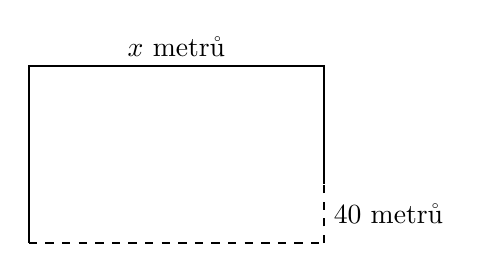
\begin{tikzpicture}[scale=0.75]
            \draw[thick] (0,0)--(0,3)--(5,3)--(5,1);
            \draw[dashed, thick] (0,0)--(5,0);
            \draw[dashed, thick] (5,0)--(5,1);

            \node[above] at (2.5,3) {$x$ metrů};
            \node[right] at (5,0.5) {$40$ metrů};
        \end{tikzpicture}
    \end{center}

    Pro $x\in(0;160)$:

    \begin{tasks}(1)
        \task Vyjádřete v $\mathrm{m}^2$ rozlohu výběhu $S$ v závislosti na $x$.
        \task Určete všechny hodnoty $x$, pro které bude mít výběh rozlohu alespoň
        $7\,000\,\mathrm{m}^2$.
        \task Vypočítejte největší možnou rozlohu výběhu.
    \end{tasks}

\end{exercise}




\end{document}